% vim: set filetype=tex spell :

%CubeSat Chapter 
\chapter{Hardware Implementation of the \acf{ACDS}}

\label{ch:CubeSatHardware}

\section{Mechanical Configuration of the \acf{ARC}}

The \ac{ARC} uses the same board geometry as the CubeSat Kit\cite{CSK} hardware making it compatible with other CubeSat hardware. The \ac{ACDS} board has the same overall outline and hole pattern but it has 4 notches cut out to accommodate the Z-axis torquers and torquer standoffs. Additionally, there is a bump-out for the \ac{USB} connector so that it can be closer to the access port to allow a \ac{USB} cable to be easily plugged in.

\Cref{fig:arcMech} shows the mechanical design of the \ac{ARC}. The design has a central board stack with solar panels and rails attached to rings that are on the top and bottom of the board stack. The \ac{ACDS} board is located 3rd from the bottom of the stack. This puts it in the center of the board stack. Because the solar cells cover all of the side faces except a small strip in the center this makes the \ac{ACDS} board the only place to put access port connections. The separation switch connections are also located on the \ac{ACDS} board as the separation switch is attached to one of the torquer standoff.

\begin{figure}[!ht]
    \centering
    \begin{minipage}{0.31\linewidth}
        \begin{tikzpicture}[remember picture,node distance=1em]
            \def\sysx{0.8}
            \node[anchor=south west,inner sep=0] (image) at (0,0) {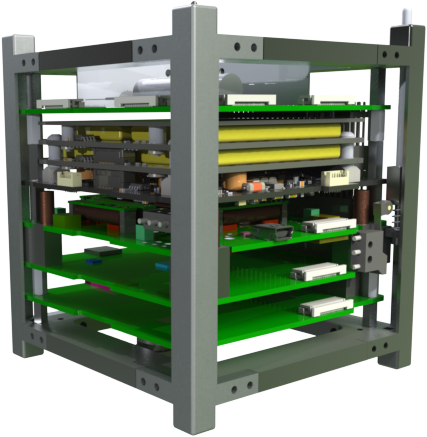
\includegraphics[width=\linewidth]{cubesat-core}};
            \begin{scope}[x={(image.south east)},y={(image.north west)}]
                % define destination coordinates
                \path (\sysx,0.751) coordinate (LEDL)
                      (\sysx,0.633) coordinate (EPS)
                      (0.86,0.55) coordinate (Z1tq)
                      (0.12,0.55) coordinate (Z2tq)
                      (0.3,0.52) coordinate (Xtq)
                      (\sysx,0.465)  coordinate (ACDS)
                      (0.9,0.4)  coordinate (sep)
                      (\sysx,0.366)  coordinate (COMM)
                      (\sysx,0.281)  coordinate (IMG);
              %draw axis
                \path (0.1,0.12) coordinate (axOrig);
                \draw[->,blue,very thick] (axOrig) to +(-21:0.1) coordinate (X);
                \node[blue,right of=X] (Xl) {X};
                \draw[->,magenta,very thick] (axOrig) to +(196:0.1) coordinate (Y);
                \node[magenta,left of=Y] (Yl) {Y};
                \draw[->,red,very thick] (axOrig) to +(-90:0.1) coordinate (Z);
                \node[red,below of=Z] (Zl) {Z};
              \end{scope}
        \end{tikzpicture}
    \end{minipage}\begin{minipage}{0.65\linewidth}
        \begin{itemize}\setlength{\parskip}{0pt}
            \item[\kern-2em] \tikz[na] \coordinate (LEDLi); \acf{LEDL}
            \item[\kern-2em] \tikz[na] \coordinate (EPSi); \acf{EPS}
            \item[\kern-2em] \tikz[na] \coordinate (ACDSi); \acf{ACDS}
            \item[\kern-2em] \tikz[na] \coordinate (sepi); Separation switch
            %\item[\kern-2em] \tikz[na] \coordinate (ppi); Pull Pin
            \item[\kern-2em] \tikz[na] \coordinate (COMMi); \acf{COMM}
            \item[\kern-2em] \tikz[na] \coordinate (IMGi); \acf{IMG}
        \end{itemize}
    \end{minipage}

    \begin{tikzpicture}[overlay,remember picture]
            \path[->,red,very thick] (LEDLi) edge (LEDL);
            \path[->,red,very thick] (EPSi) edge (EPS);
            \path[->,red,very thick] (ACDSi) edge (ACDS);
            \path[->,red,very thick] (sepi) edge (sep);
            \path[->,red,very thick] (COMMi) edge (COMM);
            \path[->,red,very thick] (IMGi) edge (IMG);
            %draw axis
    \end{tikzpicture}
    \caption{The \acs{ARC} mechanical setup}
    \label{fig:arcMech}
\end{figure}

The components shown in \cref{fig:arcMech} are as follows:

\begin{description}
    \item[\acs{LEDL}] one of the \acp{SMO} on \ac{ARC} is to ``Characterize the thermal and vibration environment inside the launch vehicle from ignition to orbit insertion.''\cite{ARCweb} The \ac{LEDL} does this by using a separate battery to operate during the launch phase and log data from accelerometers and temperature sensors.
    \item[\acs{EPS}] The solar cells provide power for the \ac{ARC} which is stored and regulated by the \ac{EPS}
    \item[\acs{ACDS}] one of the \acp{SMO} on \ac{ARC} is to ``Validate a novel low power \acf{ACDS}.'' \cite{ARCweb}
    \item[Separation Switch] is screwed into one of the torquer standoffs and cuts off power to the CubeSat when it is in the \ac{PPOD}.
    \item[\acs{COMM}] allows for two way communication with the ground. A 9600bps command/beacon up/down link and a 38400bps data down link are used.
    \item[\acs{IMG}] one of the \acp{SMO} on \ac{ARC} is to ``Validate a high bandwidth communication system by obtaining images of changing snow/ice coverage in arctic regions.''\cite{ARCweb}
\end{description}

For clarity the \acp{SPB} are not shown in\cref{fig:arcMech}. The \acp{SPB} are attached to mounting holes in the rails and are the outer faces of the \ac{ARC}. In addition to the solar cells the \acp{SPB} also contain sensors that are used by the \ac{LEDL} and \ac{ACDS}. \Cref{fig:SPB} shows the back side of a side \ac{SPB} with the sensors labeled. The top and bottom \acp{SPB} are similar to the side \acp{SPB} except they lack accelerometers and have parts for the antennas and antenna deployment.

\begin{figure}[!ht]
    \centering
    \begin{minipage}{0.35\linewidth}
        \begin{tikzpicture}[remember picture] 
            \node[anchor=south west,inner sep=0] (image) at (0,0) {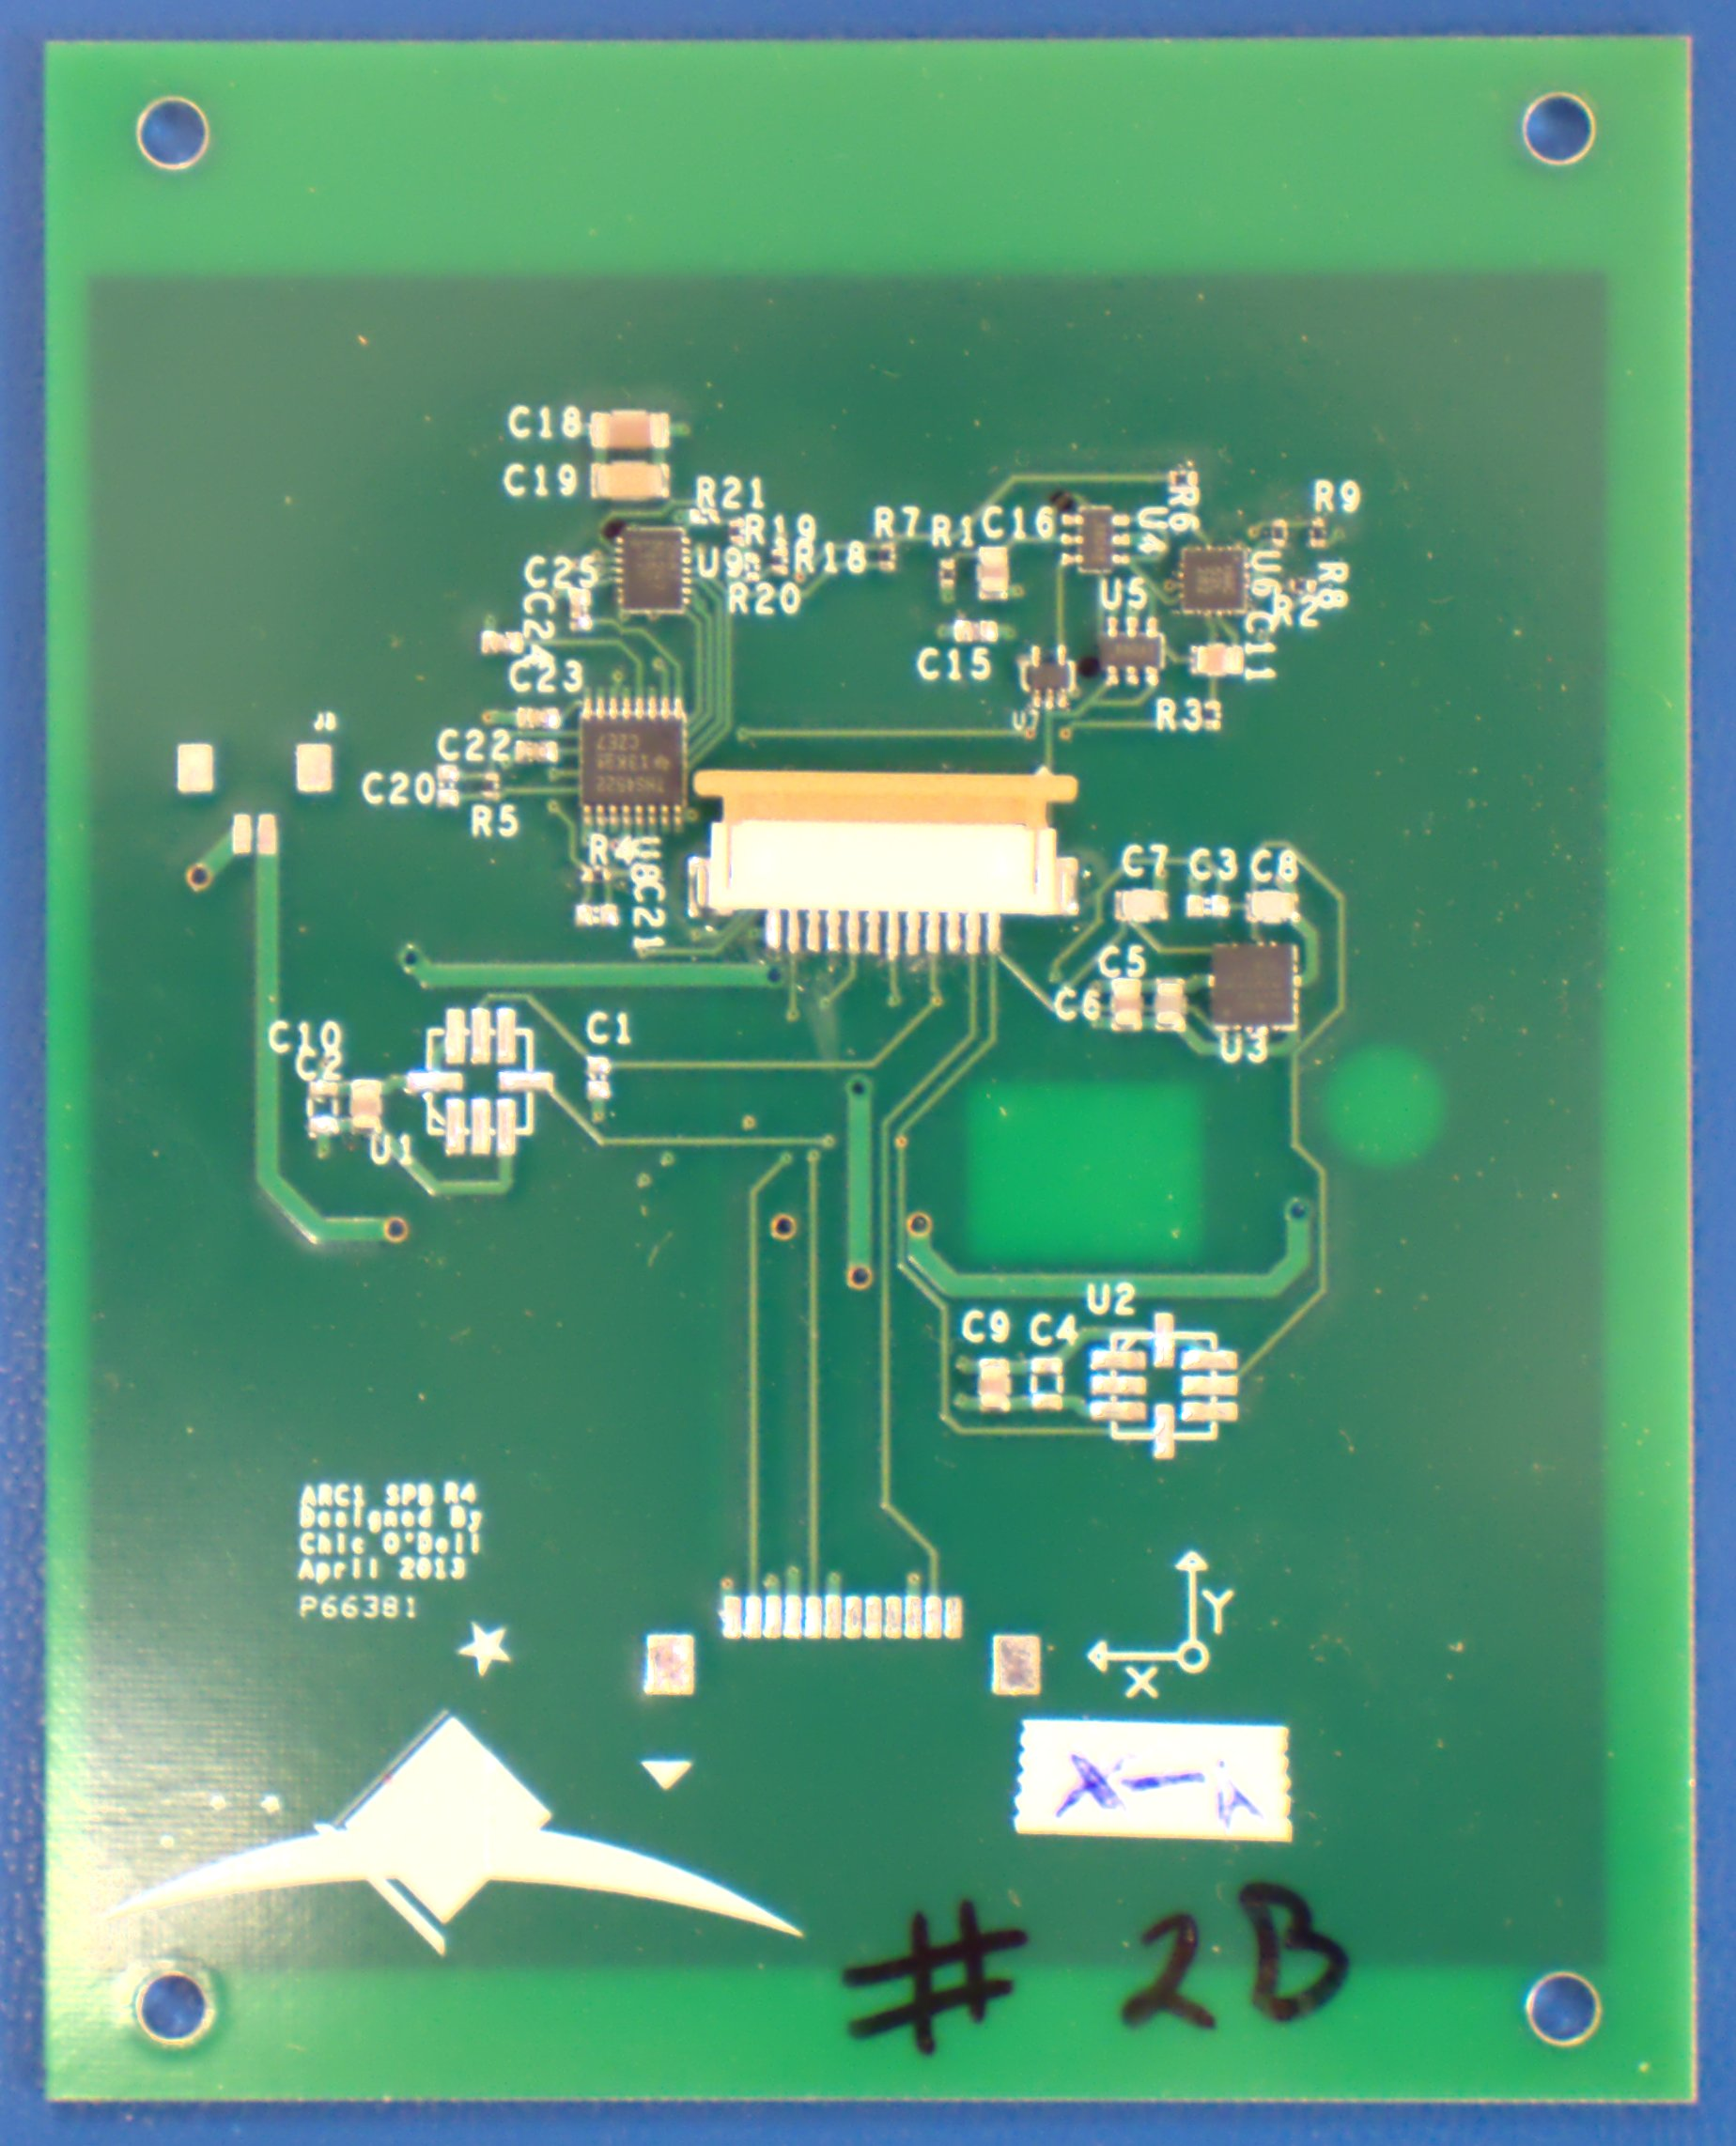
\includegraphics[width=\linewidth]{SPB}};
            \begin{scope}[x={(image.south east)},y={(image.north west)}]
                \path (0.715,0.74) coordinate (MAG)
                      (0.395,0.72) coordinate (ADC)
                      (0.395,0.65) coordinate (AMP)
                      (0.745,0.525) coordinate (ACC)
                      (0.615,0.58) coordinate (DAT);
              \end{scope}
        \end{tikzpicture}
    \end{minipage}\begin{minipage}{0.30\linewidth}
        \vspace{1em}
        \begin{itemize}\setlength{\parskip}{0pt}
            \item[\kern-0.2em] \tikz[na] \coordinate (MAGi); Magnetometer
            \item[\kern-0.2em] \tikz[na] \coordinate (ADCi); \acs{ADC}
            \item[\kern-0.2em] \tikz[na] \coordinate (AMPi); Amplifier
            \item[\kern-0.2em] \tikz[na] \coordinate (DATi); Data Connector
            \item[\kern-0.2em] \tikz[na] \coordinate (ACCi); Accelerometer
        \end{itemize}
        \vspace{4em}
    \end{minipage}

    \begin{tikzpicture}[overlay,remember picture]
            \path[->,red,very thick] (MAGi) edge (MAG);
            \path[->,red,very thick] (ADCi) edge (ADC);
            \path[->,red,very thick] (AMPi) edge (AMP);
            \path[->,red,very thick] (ACCi) edge (ACC);
            \path[->,red,very thick] (DATi) edge (DAT);
    \end{tikzpicture}
    
    \caption{Reverse side of the Solar Panel Board showing magnetometer}
    \label{fig:SPB}
\end{figure}

\subsection{\acl{ARC} Hardware}

\begin{figure}[!ht]
    \centering
    \begin{minipage}{0.35\linewidth}
        \begin{tikzpicture}[remember picture,node distance=0.5em] 
            \node[anchor=south west,inner sep=0] (image) at (0,0) {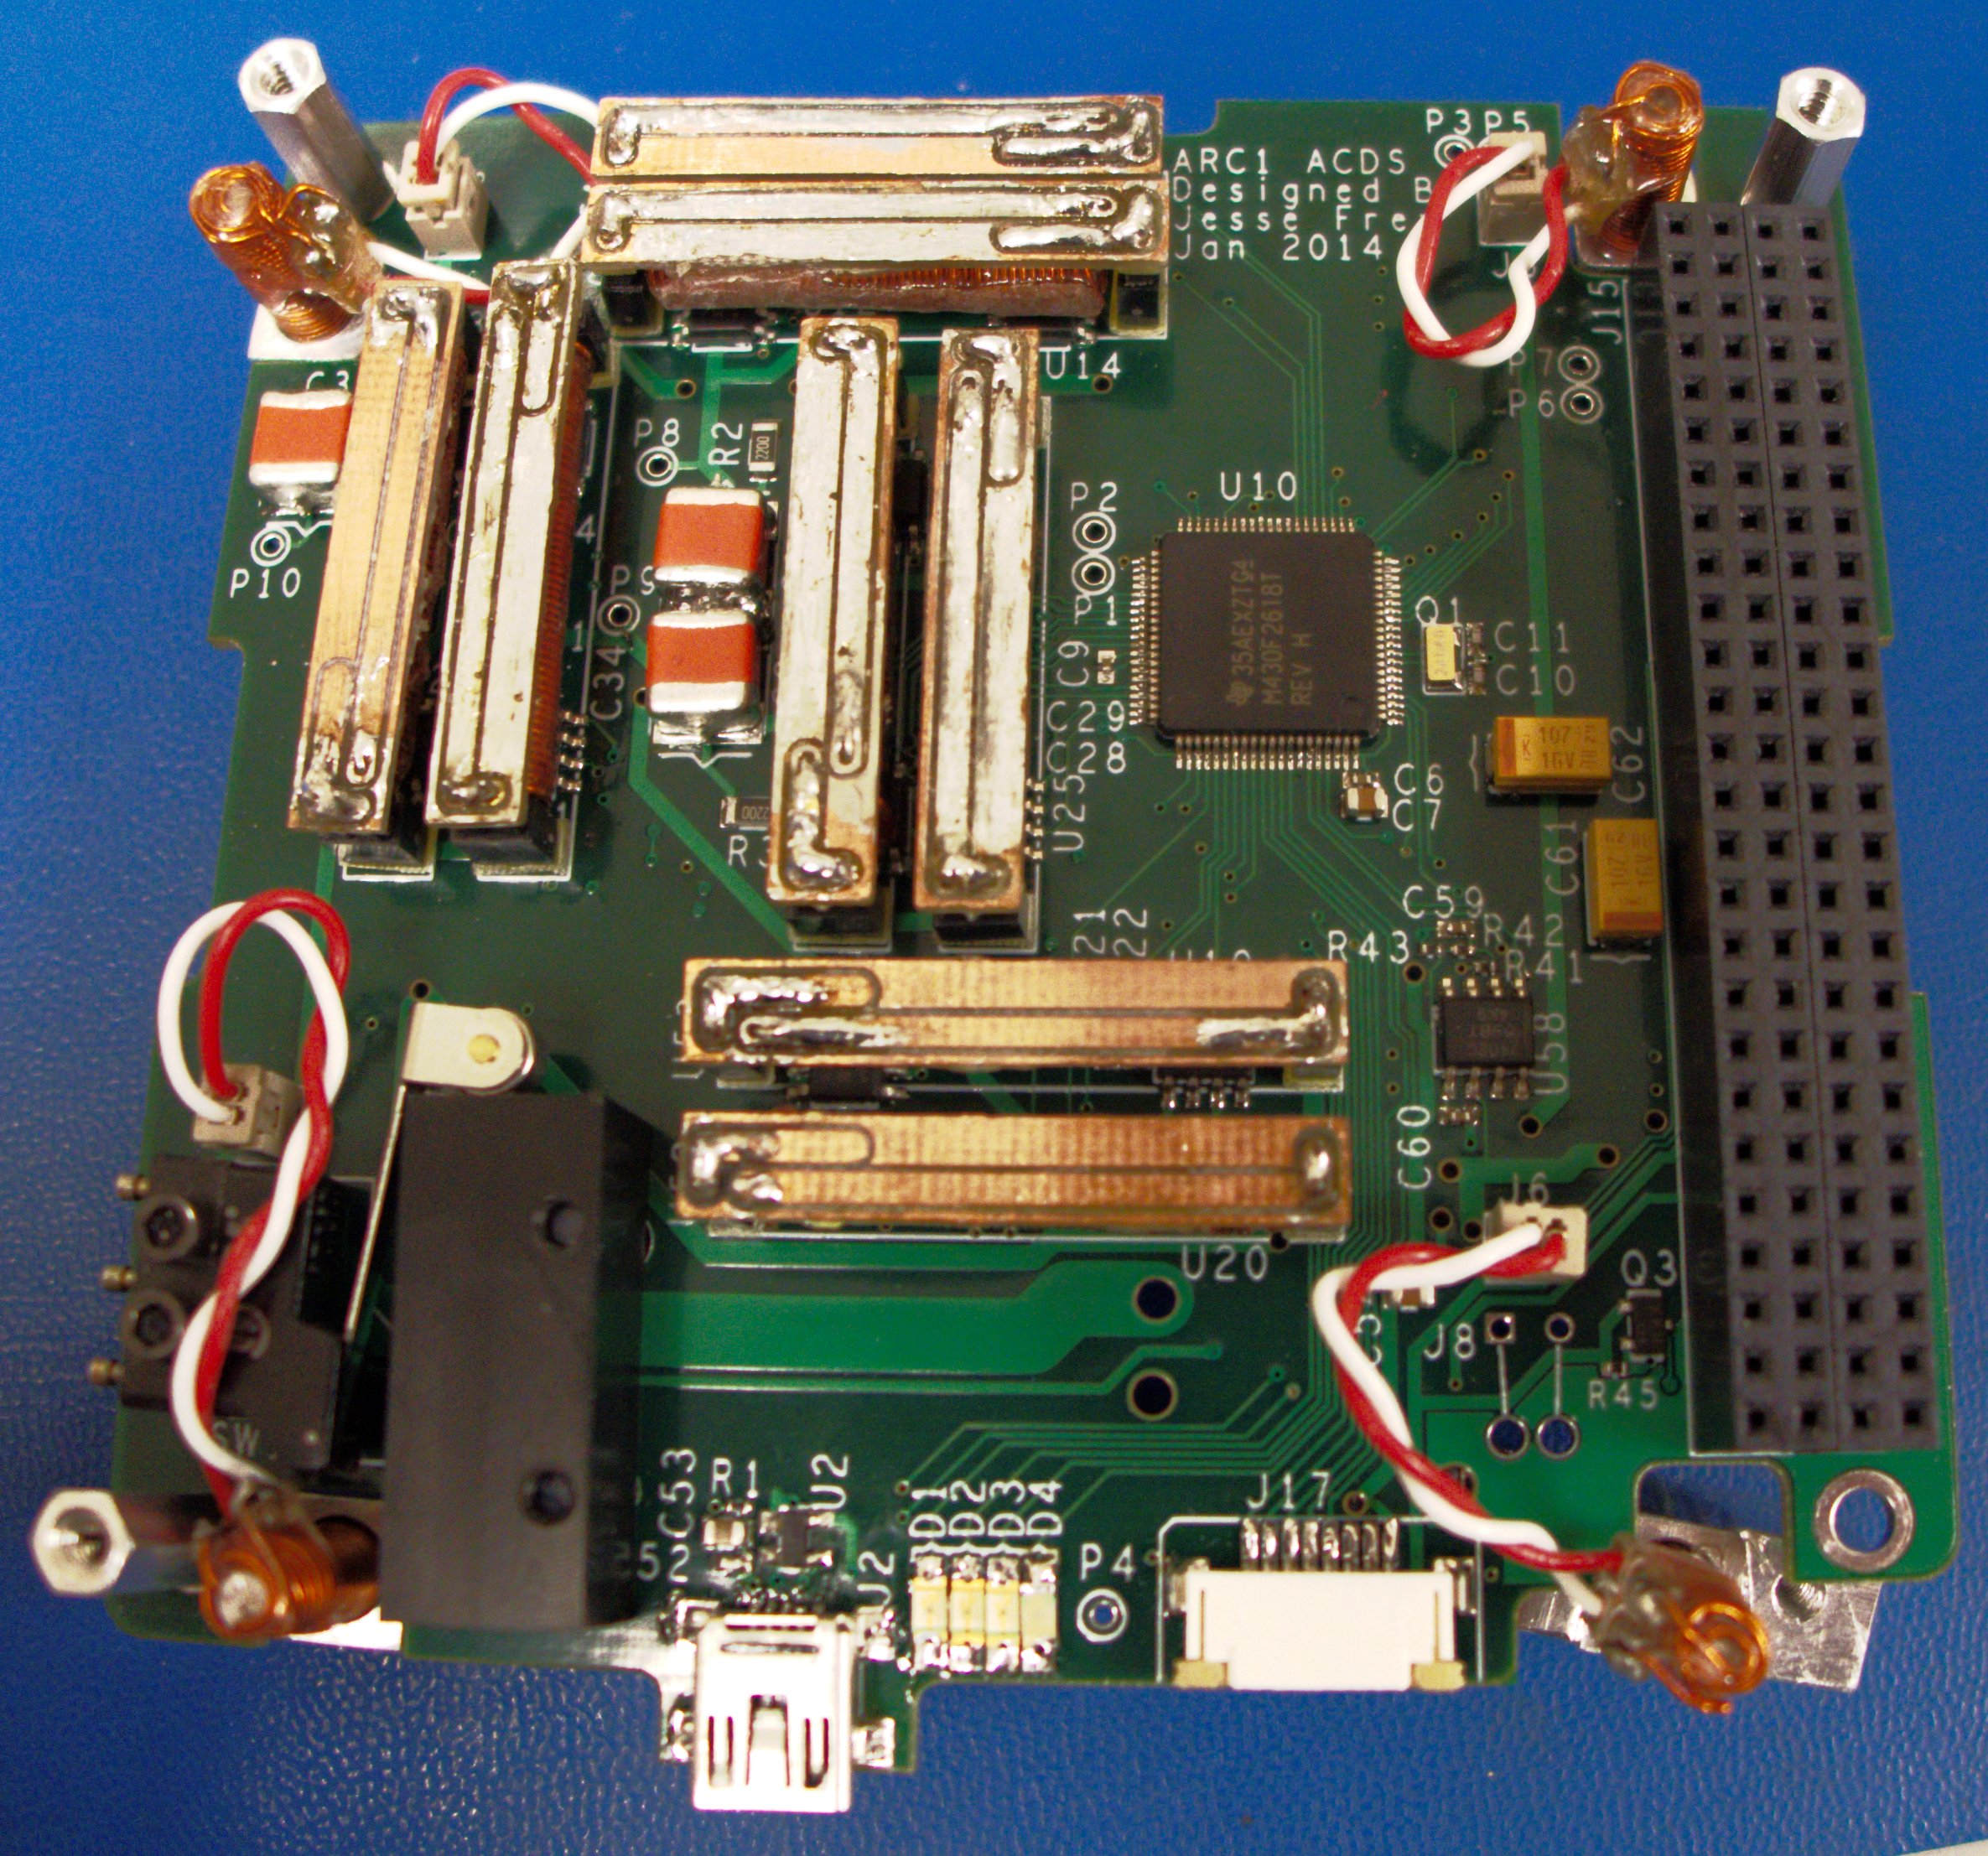
\includegraphics[width=\linewidth]{ACDS-board-photo}};
            \begin{scope}[x={(image.south east)},y={(image.north west)}]
                \path (0.30,0.27) coordinate (PP)
                      (0.38,0.07) coordinate (USB)
                      (0.46,0.70) coordinate (TqX1)
                      (0.41,0.70) coordinate (TqX2)
                      (0.22,0.70) coordinate (TqX3)
                      (0.25,0.70) coordinate (TqX4)
                      (0.45,0.90) coordinate (TqY1)
                      %(0.45,0.89) coordinate (TqY1)
                      (0.45,0.93) coordinate (TqY2)
                      (0.50,0.40) coordinate (TqY3)
                      (0.50,0.49) coordinate (TqY4)
                      (0.15,0.14) coordinate (TqZ1)
                      (0.14,0.88) coordinate (TqZ2)
                      (0.85,0.92) coordinate (TqZ3)
                      (0.87,0.14) coordinate (TqZ4);
              %draw axis
                %\path (0.15,0.72) coordinate (axOrig);
                %\draw[->,red,very thick] (axOrig) to +(-88.3:0.1) coordinate (X);
                %\node[red,below of=X] (Xl) {X};
                %\draw[->,magenta,very thick] (axOrig) to +(180.5:0.1) coordinate (Y);
                %\node[magenta,left of=Y] (Yl) {Y};
                %\draw[->,red,very thick] (axOrig) to +(-90:0.1) coordinate (Z);
                %\node[red,below of=Z] (Zl) {Z};
              \end{scope}
        \end{tikzpicture}
    \end{minipage}\begin{minipage}{0.50\linewidth}
        \vspace{1em}
        \begin{itemize}\setlength{\parskip}{0pt}
            \item[\kern-0.2em] \tikz[na] \coordinate (TqXi); X torquers
            \item[\kern-0.2em] \tikz[na] \coordinate (TqYi); Y torquers
            \item[\kern-0.2em] \tikz[na] \coordinate (TqZi); Z torquers
            \item[\kern-0.2em] \tikz[na] \coordinate (PPi); Pull Pin
            \item[\kern-0.2em] \tikz[na] \coordinate (USBi); \acf{USB} connection
        \end{itemize}
        \vspace{4em}
    \end{minipage}

    \begin{tikzpicture}[overlay,remember picture]
            \path[->,blue,very thick] (PPi) edge (PP);
            \path[->,blue,very thick] (USBi) edge (USB);
            \path[->,red,very thick] (TqXi) edge (TqX1);
            %\path[->,red,very thick] (TqXi) edge (TqX2);
            \path[->,red,very thick] (TqXi) edge (TqX3);
            %\path[->,red,very thick] (TqXi) edge (TqX4);
            \path[->,magenta,very thick] (TqYi) edge (TqY1);
            %\path[->,magenta,very thick] (TqYi) edge (TqY2);
            \path[->,magenta,very thick] (TqYi) edge (TqY3);
            %\path[->,magenta,very thick] (TqYi) edge (TqY4);
            \path[->,black,very thick] (TqZi) edge (TqZ1);
            \path[->,black,very thick] (TqZi) edge (TqZ2);
            \path[->,black,very thick] (TqZi) edge (TqZ3);
            \path[->,black,very thick] (TqZi) edge (TqZ4);
    \end{tikzpicture}
    \caption{The \ac{ARC} \ac{ACDS} board}
    \label{fig:boardPhoto}
\end{figure}

In addition to the \ac{ACDS} hardware the \ac{ACDS} board also contains the pull pin and \ac{USB} connection. This is located on the \ac{ACDS} board because it is the only board that can connect to the access port. The pull pin and \ac{USB} connection connect directly to the header and are not connected to the core \ac{ACDS} hardware. 

The Z-axis torquers are housed inside the standoffs which are located on the four corners of the board. To accommodate the standard board shape has been modified to accommodate the torquers. This is visible in \cref{fig:boardPhoto}. The notches are designed to fit the torque standoffs and help keep them in the proper orientation. The torquers fit into a hole drilled into the standoffs and are held in place with epoxy. 

The standard board shape has also been modified to allow the \ac{USB} connector to be placed closer to the access port so that the \ac{USB} cable can be easily plugged in. This is also visible in \cref{fig:boardPhoto}.

\subsection{Bus Communication}

The subsystems of the \ac{ARC} will communicate with each other using the ARCBus. The ARCBus consists of shared connections between the subsystems to transmit commands and data. The ARCBus will primary used by the \ac{ACDS} to get sensor data from the \ac{LEDL} and send and receive data to the ground station through the COMM system. Commands are transmited using an \ac{I2C} bus and large blocks of data are sent using a \ac{SPI} bus which is negotiated using the \ac{I2C} bus.

\section{\acl{ACDS} System Block Diagram}

The block diagram for the CubeSat hardware used to implement the \ac{ACDS}. The hardware necessary for the \ac{ACDS} is spread over multiple subsystems of the \ac{ARC}. The \ac{ACDS} board contains the torquers, driving hardware along with the microcontroller which will run the attitude control algorithm. There is one two axis magnetometer located on each of the six of the \acp{SPB}. These are used by the \ac{ACDS} to calculate rotation rates and calculate the magnetic dipole moment required to generate the necessary torque. Spreading the magnetometers across all six faces should give some degree of noise immunity and redundancy. The \ac{LEDL} board also contains \ac{MEMS} angular rate sensors as a redundant reading of the rotation rate of the \ac{ARC}. The sensors on the \acp{SPB} are read by the \ac{LEDL} which then forwards the magnetometer and angular rate measurements to the \ac{ACDS}.

\begin{figure}[H]
    \centering
    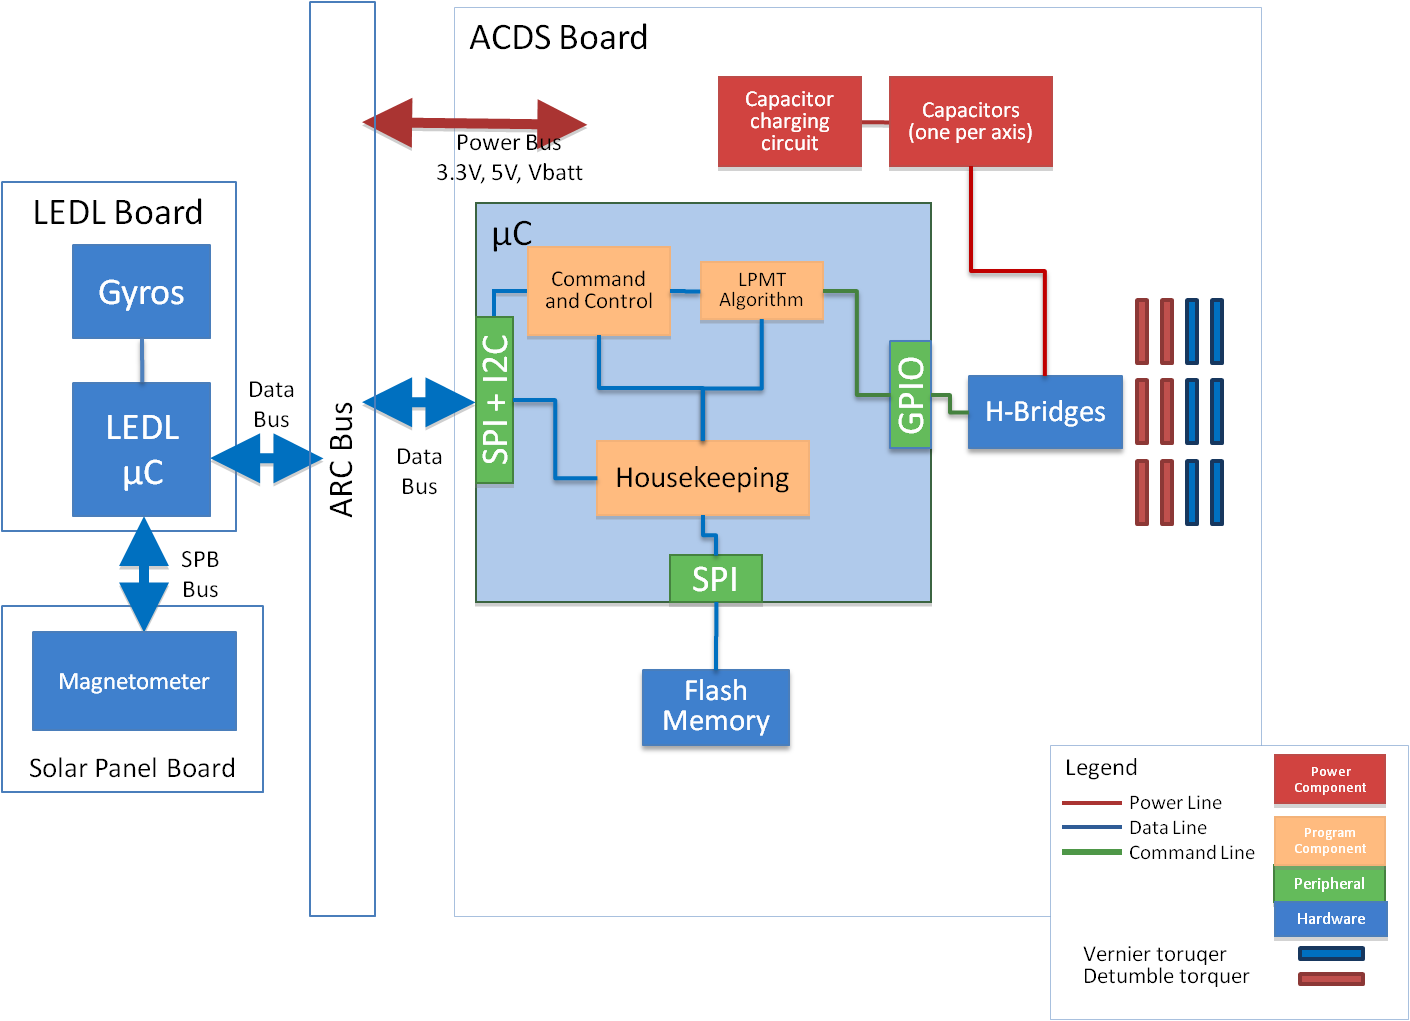
\includegraphics[width=0.8\textwidth]{Figures/Block}
    \caption{Block Diagram of the CubeSat \acs{ACDS} system}
\end{figure}


\section{Torquers}

\Cref{fig:torquers} shows the torquer locations within the \ac{ARC}. The torquers consist of a hard magnetic core surrounded with a coil of wire. There are a total of twelve torquers on the \ac{ARC}, four in each axis. The torquers are flipped using the driving circuit which causes a current pulse to flow through the coil. The driving hardware for the torquers is designed to flip one torquer in each axis every second.

\begin{figure}[!ht]
    \centering
    \begin{minipage}{0.25\linewidth}
        \begin{itemize}\setlength{\parskip}{0pt}
            \item[\kern-0.2em] Magnetometer \tikz[na] \coordinate (MAGi);
            \item[\kern-0.2em] Y torquers \tikz[na] \coordinate (YTi);
            \item[\kern-0.2em] X torquers \tikz[na] \coordinate (XTi);
            \item[\kern-0.2em] Z torquers\tikz[na] \coordinate (ZTi);
        \end{itemize}
    \end{minipage}\begin{minipage}{0.55\linewidth}
        \begin{tikzpicture}[remember picture] 
            \node[anchor=south west,inner sep=0] (image) at (0,0) {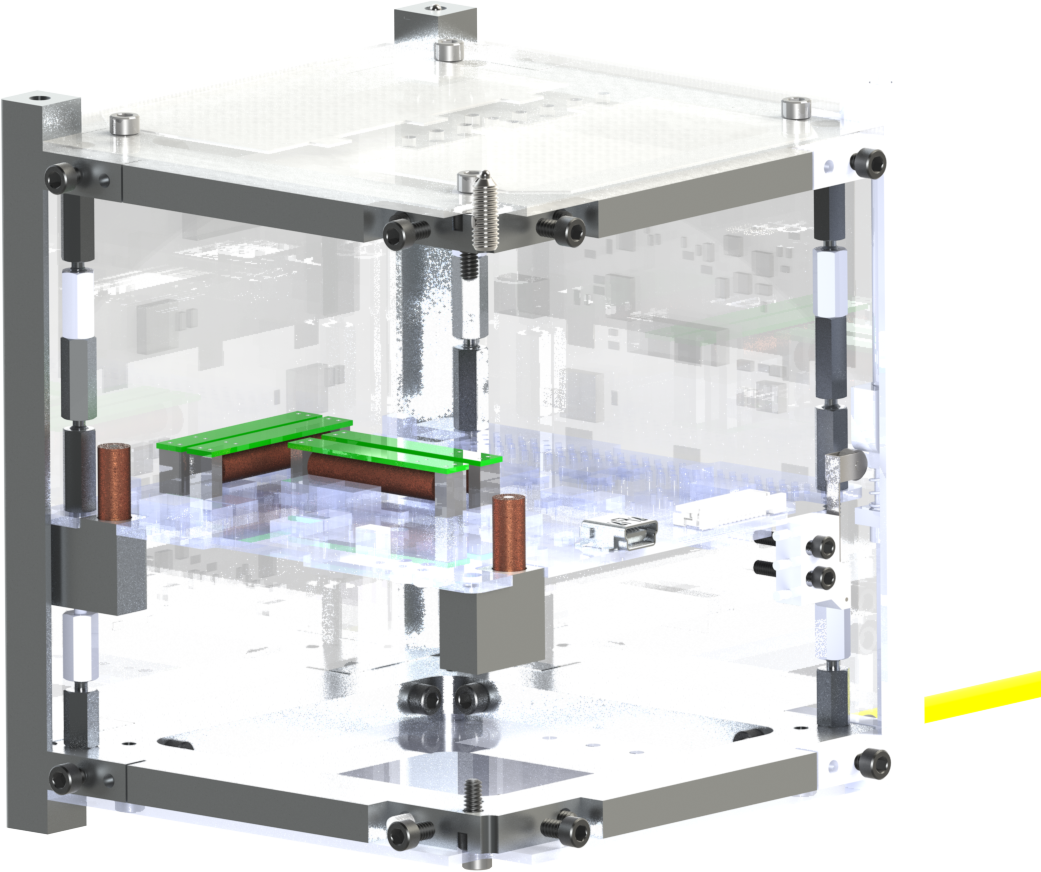
\includegraphics[width=\linewidth]{torquers}};
            \begin{scope}[x={(image.south east)},y={(image.north west)}]
                \fill[blue,fill opacity=0.3] (0.722,0.712) -- (0.74,0.709) -- (0.74,0.683) -- (0.723,0.685) -- cycle;
                \path (0.722, 0.7) coordinate (MAG)
                      (0.28,0.49) coordinate (XT)
                      (0.208,0.51) coordinate (YT)
                      (0.1,0.45) coordinate (ZT1)
                      (0.48,0.4) coordinate (ZT2);
              \end{scope}
        \end{tikzpicture}
    \end{minipage}

    \begin{tikzpicture}[overlay,remember picture]
            \path[->,red,very thick] (MAGi) edge (MAG);
            \path[->,red,very thick] (XTi) edge (XT);
            \path[->,red,very thick] (YTi) edge (YT);
            \path[->,red,very thick] (ZTi) edge (ZT1);
            \path[->,red,very thick] (ZTi) edge (ZT2);
    \end{tikzpicture}
    
    \caption{Torquer locations within the \ac{ARC}}
    \label{fig:torquers}
\end{figure}

\subsection{Cores}

The torquer cores are made of Alnico1 which is a hard magnetic material. Most magnetic torquers use either an air core or a soft magnetic core. Ideally both an air or a soft core only produce torque while a current is running through the coil. A soft core will produce more torque for the same geometry and current, however soft magnetic materials have some hysteresis that will continue to produce undesired torque after current stops flowing. Hard magnetic materials are chosen to have a large amount of hysteresis so that after the current stops flowing in the coil torque is produced. 

\subsubsection{Core Sizing}

The torquer cores from \cite{Mentch11} consisted of a large and a small pair in each axis. All torquer cores were the same size, one inch long $\sfrac{1}{16}$th inch diameter rod. The large pair was made of Alnico1 and produced a magnetic dipole moment of $0.022 \unit{A m^2}$. The small pair was proposed to have an inert core with a thin permalloy coating to give it a dipole moment of $0.00011 \unit{A m^2}$.

As discussed in \cite{Mentch11} the large cores were sized by first determining the desired torque then calculating the necessary dipole moment. Simulation was used to refine the required dipole moment. Alnico5 was the core material that had been used in prevous expariments for much larger cores. The minimum manufacturable size of alnico rods is $\sfrac{1}{16}$. It is desirable to have a length to diameter ratio greater than 10 which fixes the minimum torque that can be achieved. The torque using Alnico5 was larger then the desired torque so Alnico1 was used instead which has a lower residual induction. 

The proposed size of the small torquers was $\sfrac{1}{200}$th the torque of the alnico torquers. The fabrication of the proposed torquer was not completed and even if it had it is not clear that testing could have been done to quantify the dipole moment. In addition to fabrication and testing issues there is the problem of balancing the alnico cores. Because of theses difficulties the original design for the small torquers was dropped and an extra set of Alnico torquers was added in their place. The charge time was also shortened from 10 seconds to 1 second.

\subsubsection{Measuring Dipole Moment}

Determining the dipole moment is not an easy task as the dipole moments are quite small. I should probably do some dipole measurements and write it up.

\subsection{Coils}

The coils used to drive the torquers are made from four layers of 26 AWG wire. The current spike to flip the torquer peaks around 7A which is significantly higher than 26 AWG can handle with continuous current however, because the pulse duration is short it is not a problem.

\subsection{Drivers}

The schematic to drive a pair of torquers is shown in \cref{fig:drive}. Each pair of torquers is driven by three complimentary pairs of \acp{MOSFET}.  The \acp{MOSFET} are driven by three pairs of \ac{MOSFET} drivers which are controlled by the \ac{ACDS} microcontroller.

In the idle state all of the \acp{MOSFET} are off and the torquer coils are floating. This prevents changing magnetic fields in the torquers causing current to flow in them. To flip a torquer one end of the torquer is shorted to ground using one of the N-Channel \acp{MOSFET} and the other end is shorted to C1 using one of the P-Channel \acp{MOSFET}. After a 2ms delay the \acp{MOSFET} are switched off and C1 begins to recharge.

\begin{figure}[H]
    \centering
    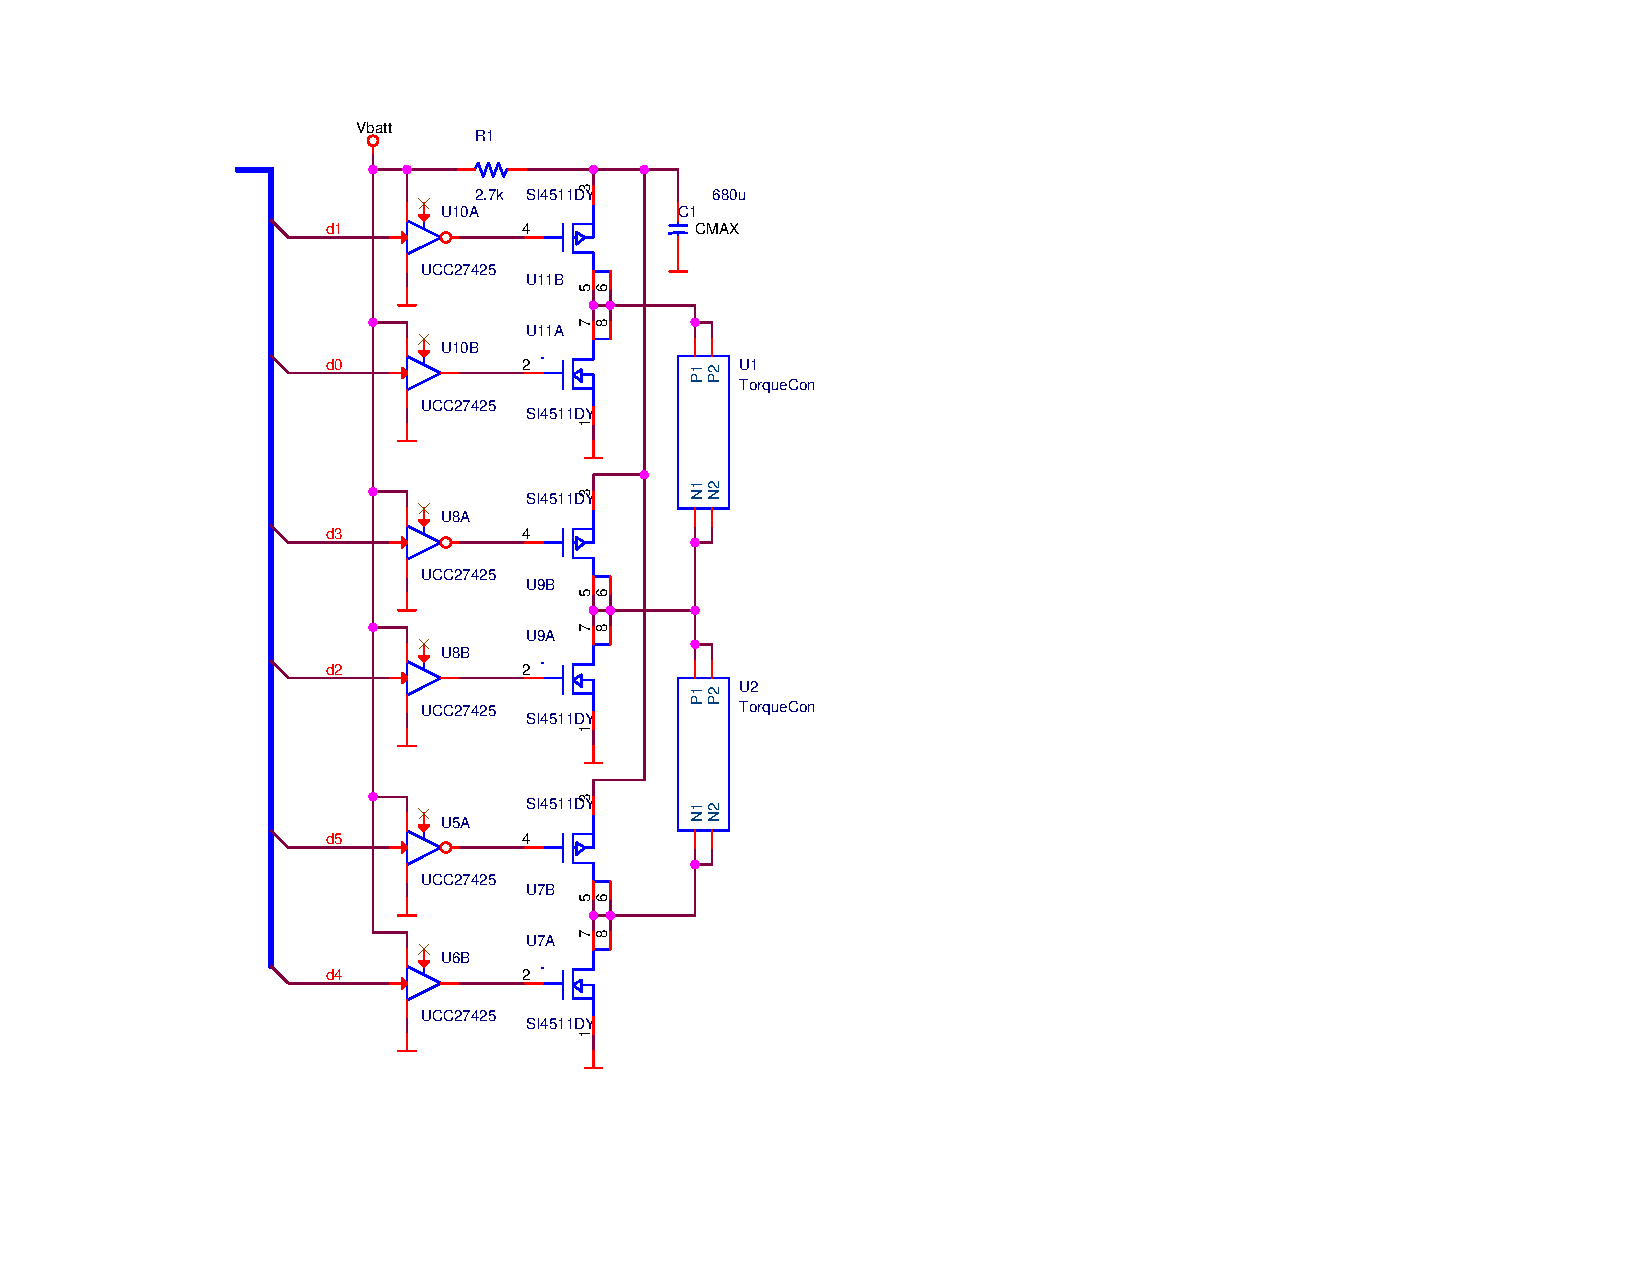
\includegraphics[width=0.5\textwidth]{Figures/driverSchematic}
    \caption{Torquer Driver schematic}
    \label{fig:drive}
\end{figure}

\subsubsection{Driving Waveform}

\begin{figure}[H]
    \centering
    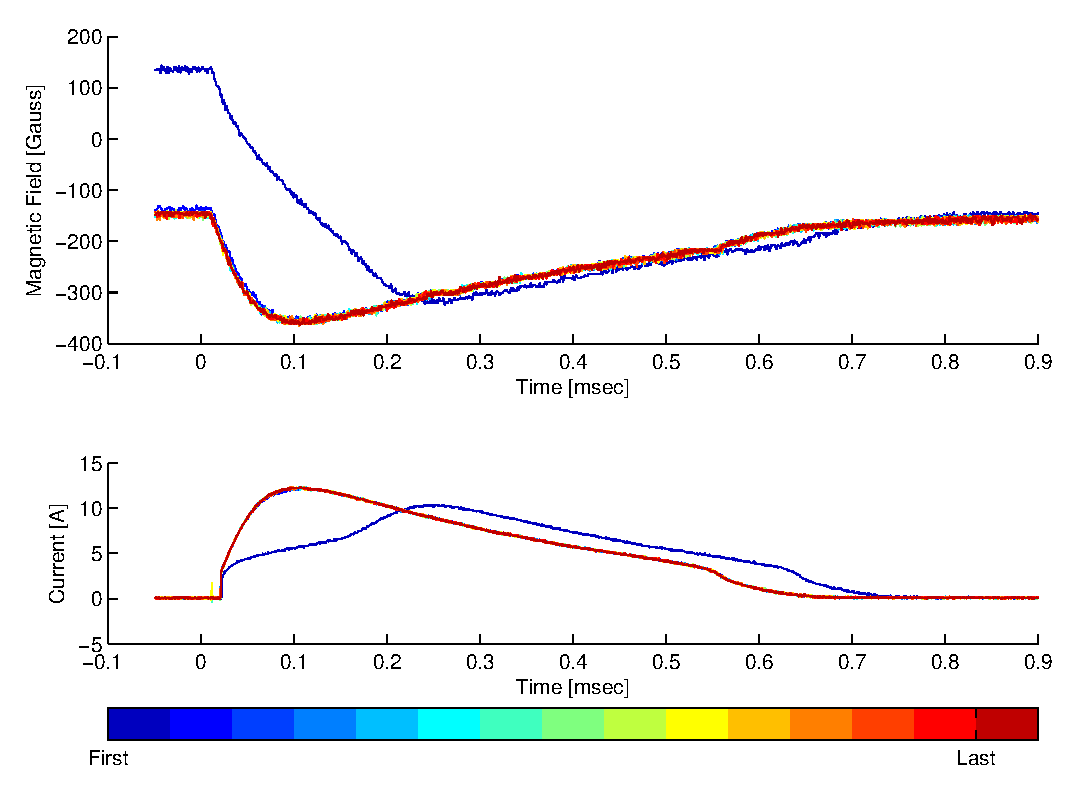
\includegraphics[width=0.7\textwidth]{torquer-waveforms}
    \caption{Torquer driving waveform showing multiple torquer flips}
    \label{fig:driveWV}
\end{figure}

\Cref{fig:driveWV} shows the driving waveform when driving a torquer multiple times in the same direction. The first flip is shown in blue and it starts at about +125 Gauss. The reset of the waveforms start at about -125 Gauss. This is because the first flip drives the torquer into saturation flipping the direction that the torquer is magnetized in.

The Current waveforms also show changes due to torquer saturation. For the first flip the current initially increases at a slower rate. This because, on the Alnico1 B-H curve, the slope is steeper closer to the B-axis resulting in a higher inductance. As the torquer reaches saturation the inductance of the torquer goes down and the rate of change of current increases. For the subsequent torquer flips the torquer is already saturated so the inductance is low and the driving current reaches its peak much faster.

\begin{figure}[H]
    \centering
    \begin{tikzpicture}[remember picture,node distance=1em]
        \def\sysx{0.8}
        \begin{pgfonlayer}{background}
            \node[anchor=south west,inner sep=0] (image) at (0,0) {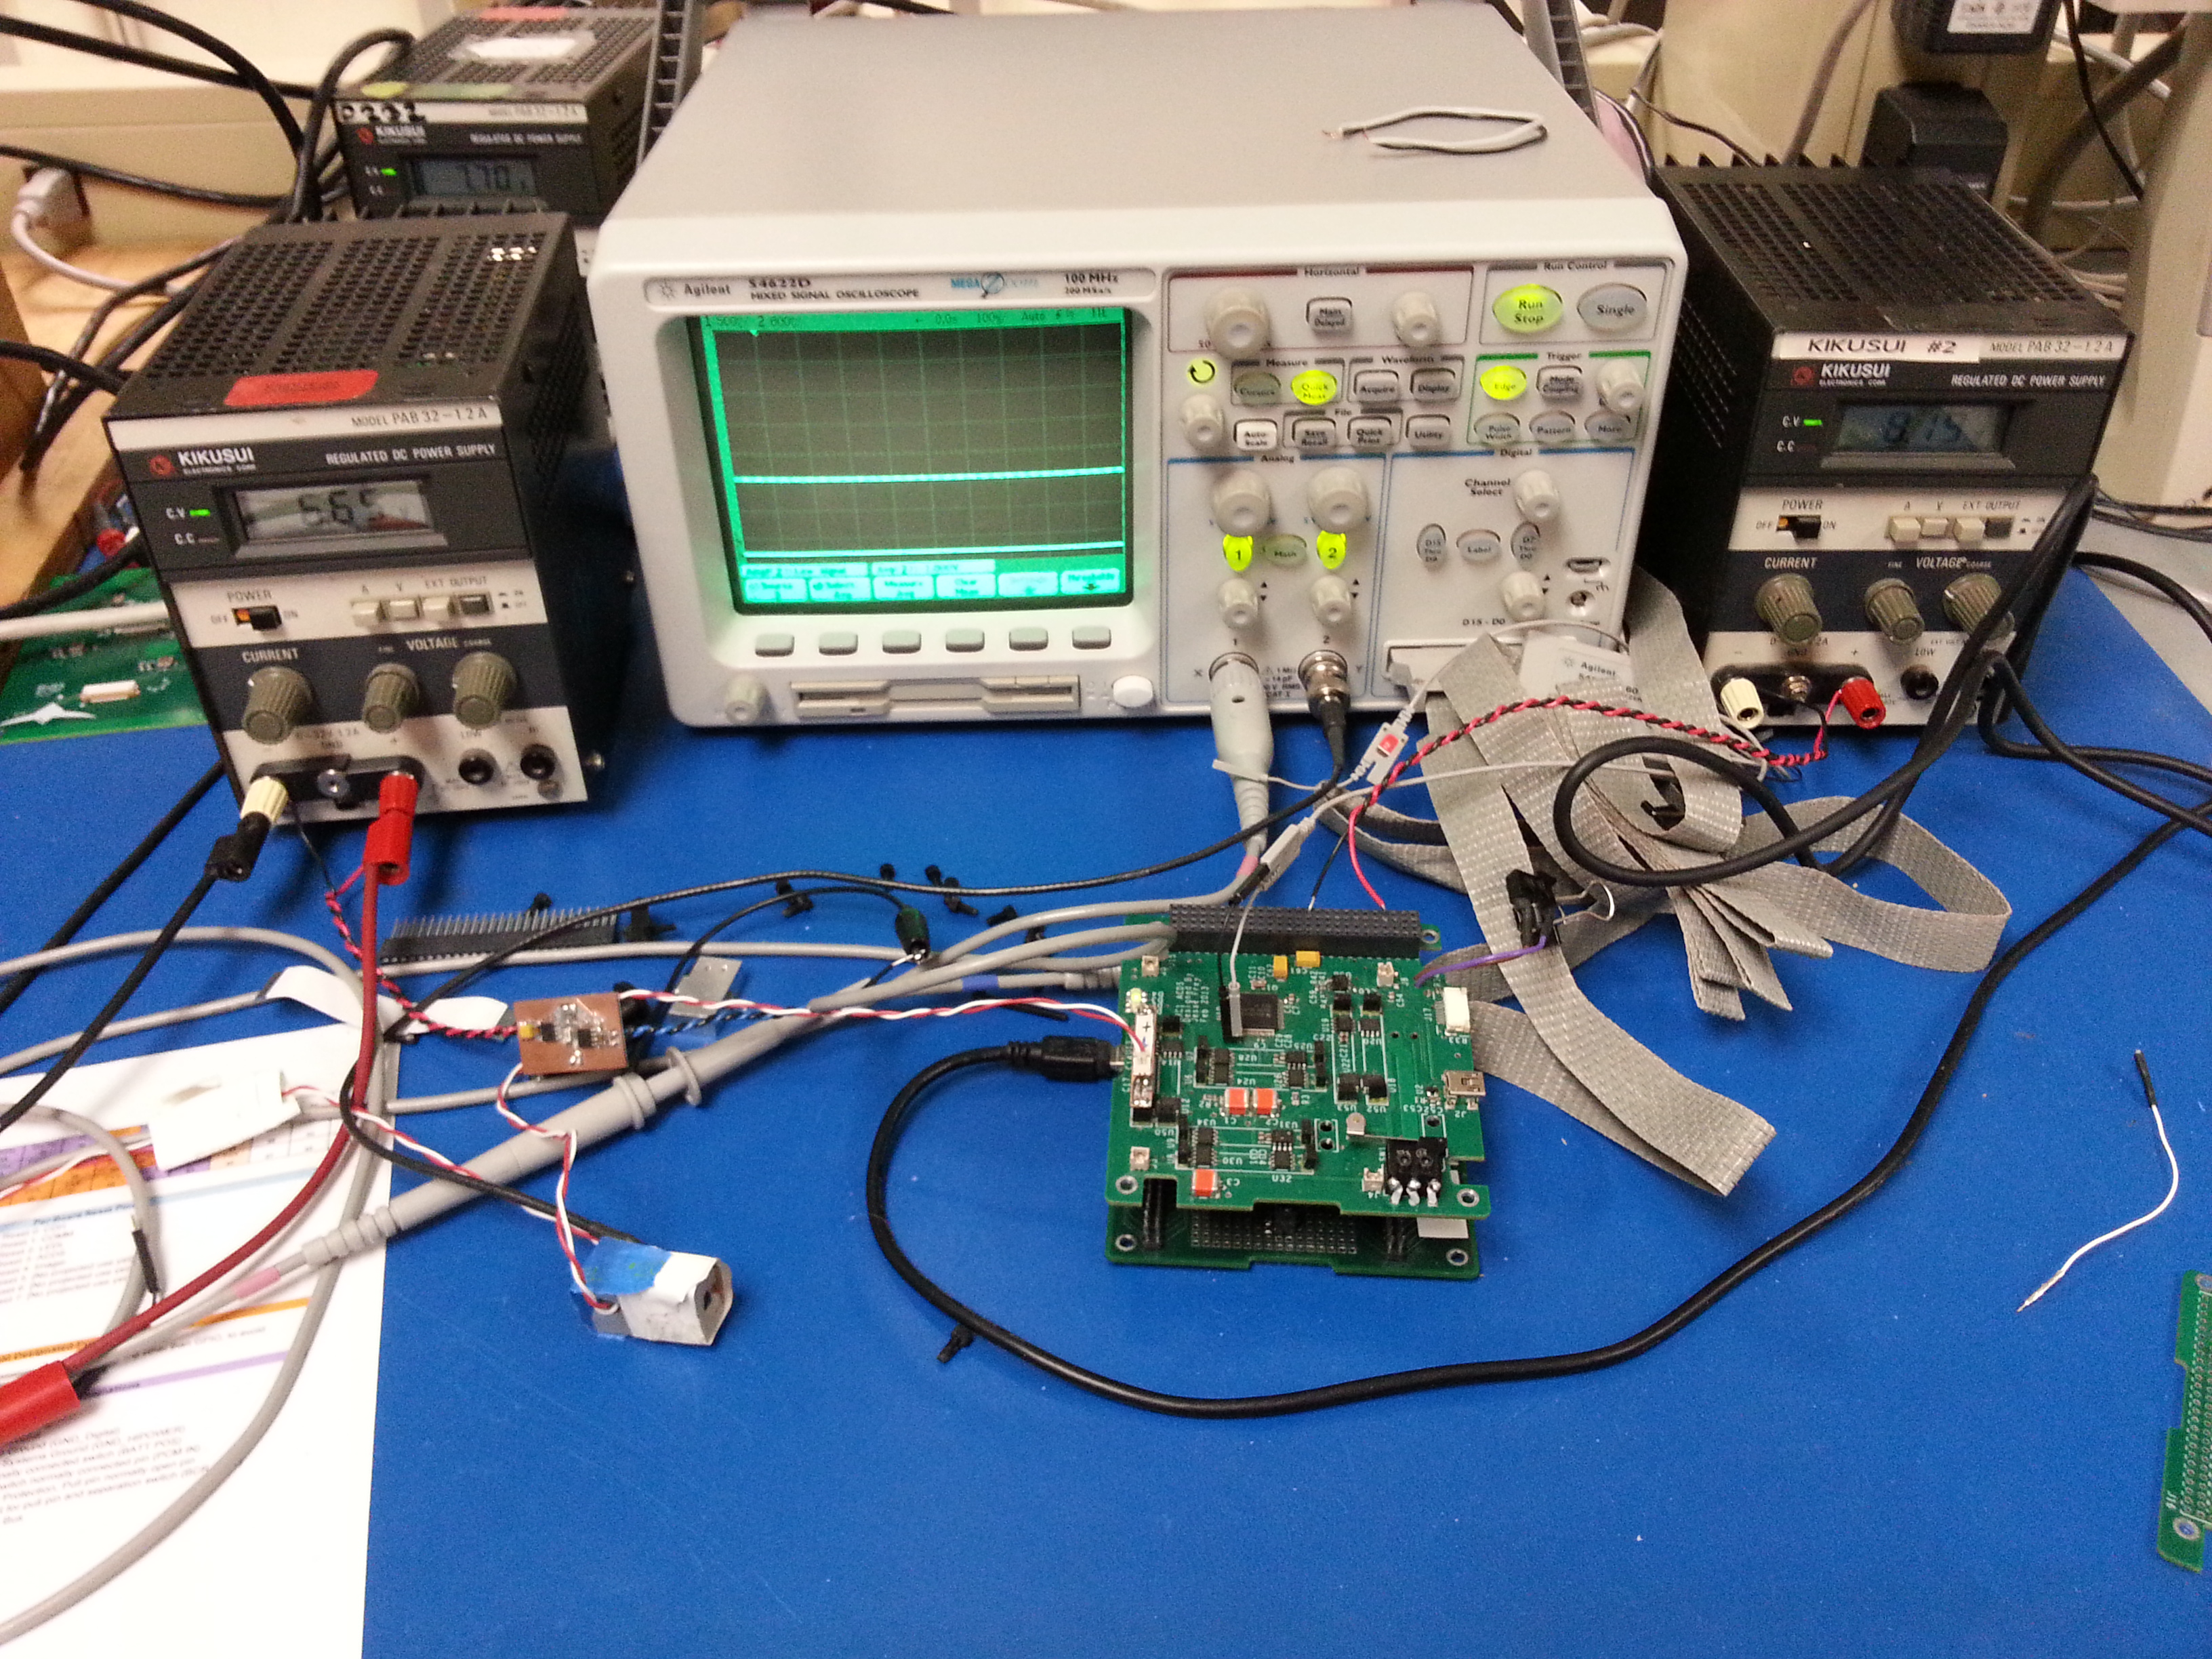
\includegraphics[width=\linewidth]{torquer-waveform-setup}};
        \end{pgfonlayer}
        %insert detail image
        \begin{scope}[x={(image.south east)},y={(image.north west)}]
            \node[inner sep=0] (detail) at (0.13,0.19) {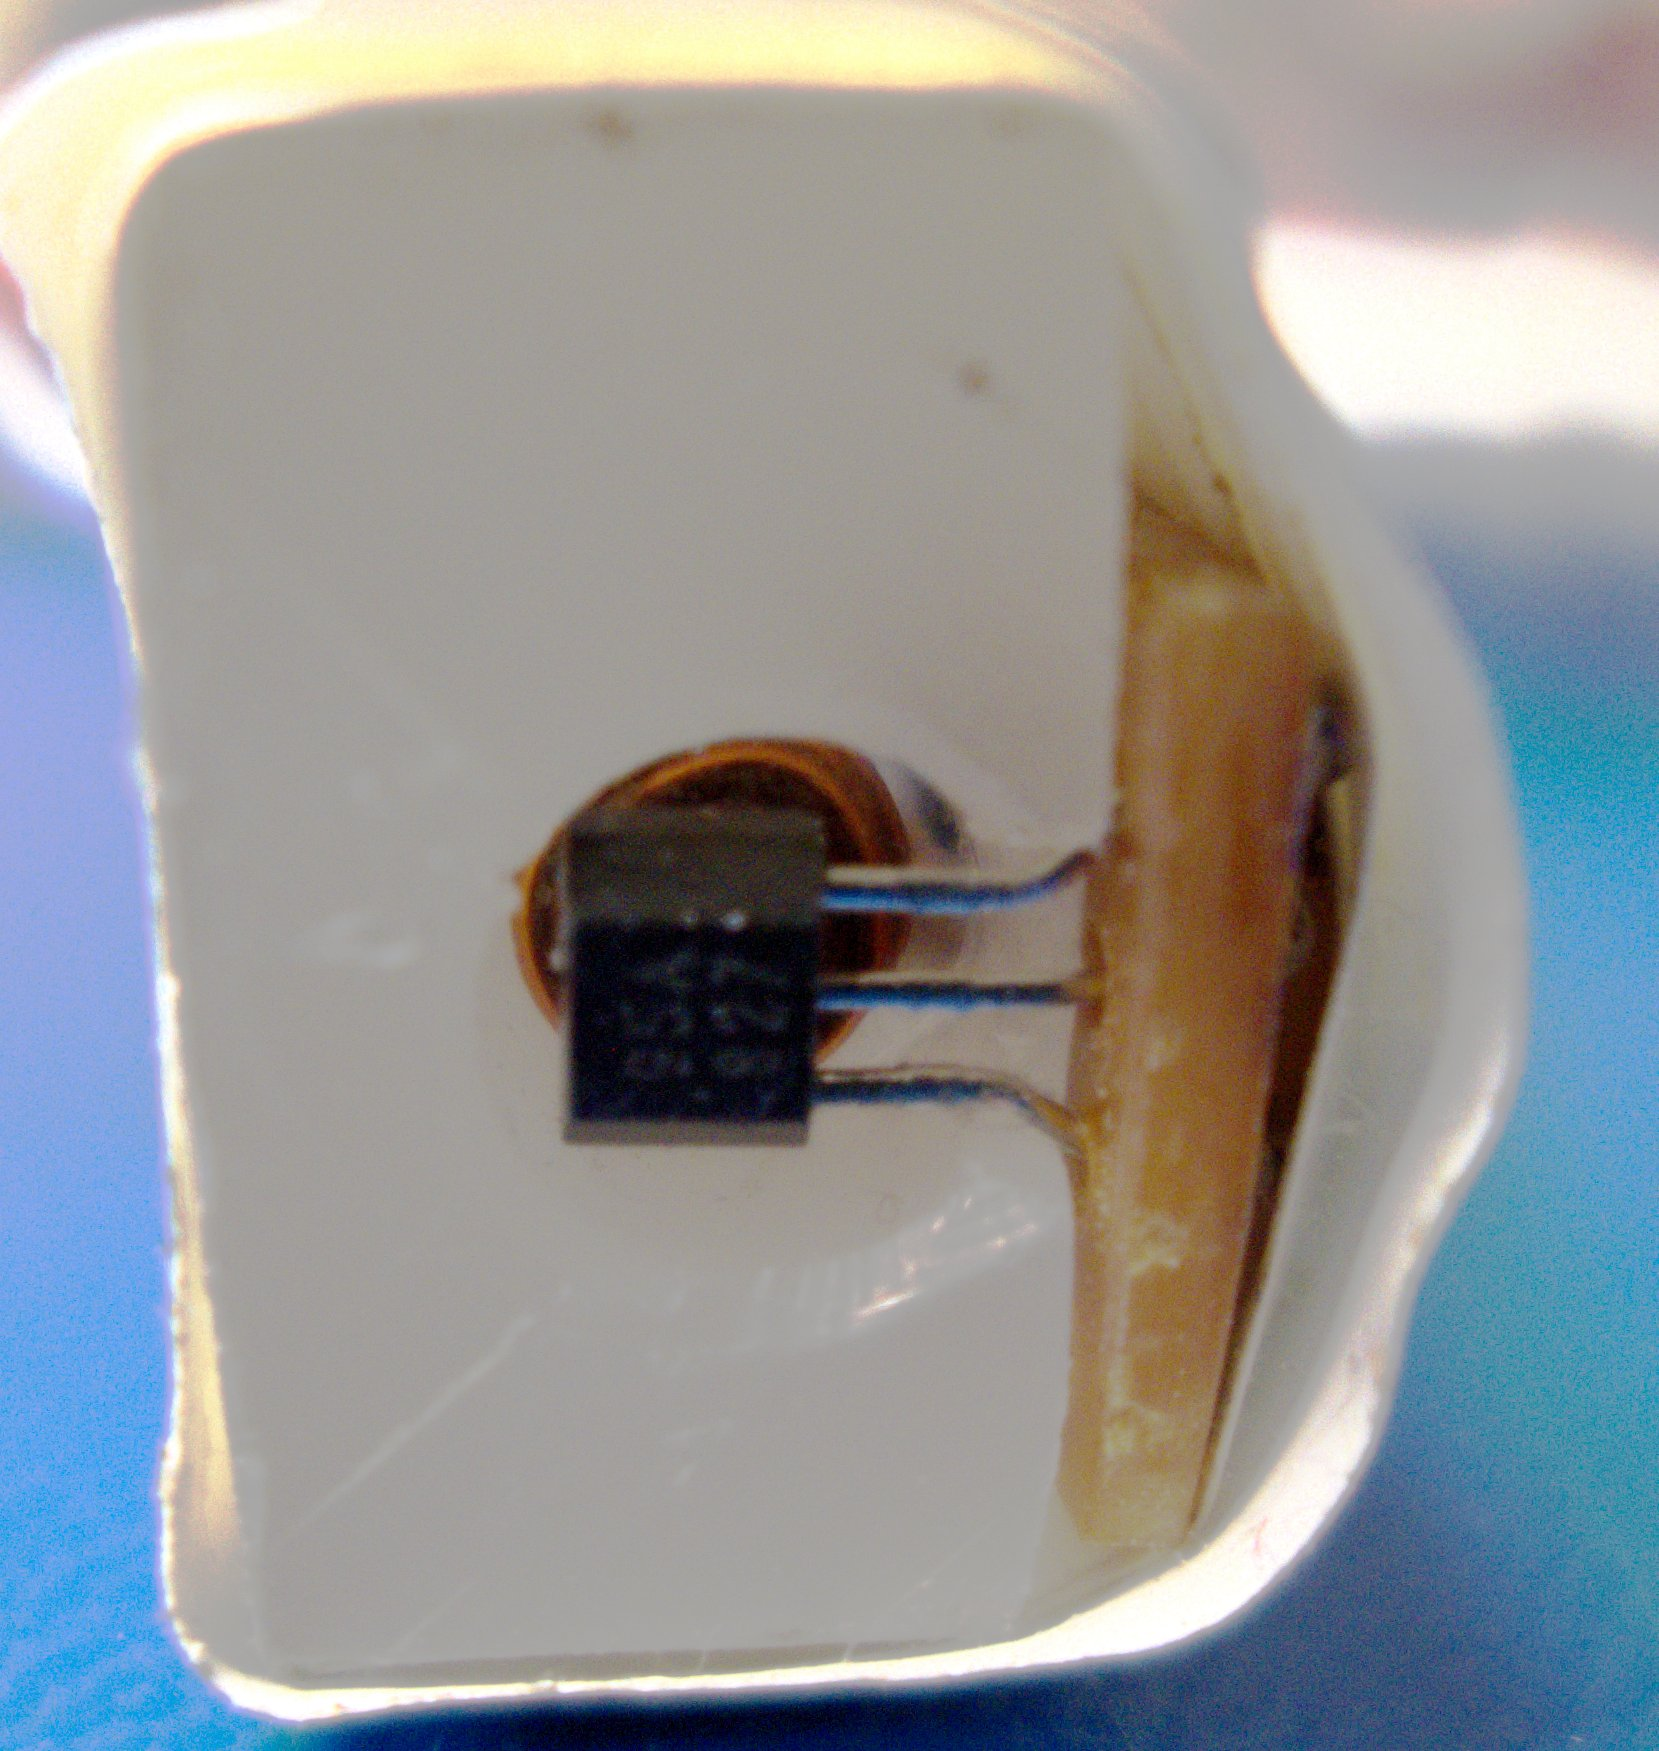
\includegraphics[width=1in,angle=-90]{testing-sensor}};
            %declare coordinates for box around sensor
            \path   (0.31,0.17) coordinate (box1)
                    (0.31,0.22) coordinate (box2)
                    (0.28,0.22) coordinate (box3)
                    (0.28,0.17) coordinate (box4);
            %draw box around sensor detail
            \draw[magenta,very thick] (detail.south east) -- (detail.south west) -- (detail.north west) -- (detail.north east) -- cycle;
            %draw box around sensor
            \draw[red,very thick] (box1) -- (box2) -- (box3) -- (box4) -- cycle;
            %draw ``expanding lines'' to detail
            \begin{pgfonlayer}{background}
                \draw[red,very thick] (box1) -- (detail.south east);
                \draw[red,very thick] (box2) -- (detail.north east);
                \draw[red,very thick] (box3) -- (detail.north west);
                \draw[red,very thick] (box4) -- (detail.south west);
            \end{pgfonlayer}
        \end{scope}
    \end{tikzpicture}
    \caption{Setup for measuring \cref{fig:driveWV,fig:satWV}. The Hall effect sensor on the end of the torquer is shown in detail}
    \label{fig:WVsetup}
\end{figure}

\Cref{fig:WVsetup} shows the hardware used to take the data for \cref{fig:driveWV,fig:satWV}. The \ac{ACDS} board was used to drive the torquers. To communicate with the \ac{ACDS} a development board was used which is plugged into the \ac{USB} cable. The torquer connects to the \ac{ACDS} board through a current sensor which is read by the oscilloscope. The torquer is placed inside a plastic housing with an attached Hall effect sensor. The hall effect sensor is located against the end of the torquer and is read by the oscilloscope. A pin on the \ac{ACDS} microcontroller is  used to trigger the scope which is automatically configured by a Matlab script which communicates with the \ac{ACDS} board and the oscilloscope.

The measured field that the Hall effect sensor reads is highly dependant on the distance from the torquer. Using the residual induction of Alnico1, 7200 Gauss \cite{AlnicoProp}, and \cite{DexterField} the magnetic field from the torquers should be 153 Gauss at 0.1 in form the face of the torquer. This is close to what is shown in \cref{fig:driveWV}. As the distance from the face increases to 0.2 and 0.3 in the field decreases to 44 and 20 Gauss respectively.

\begin{figure}[H]
    \centering
    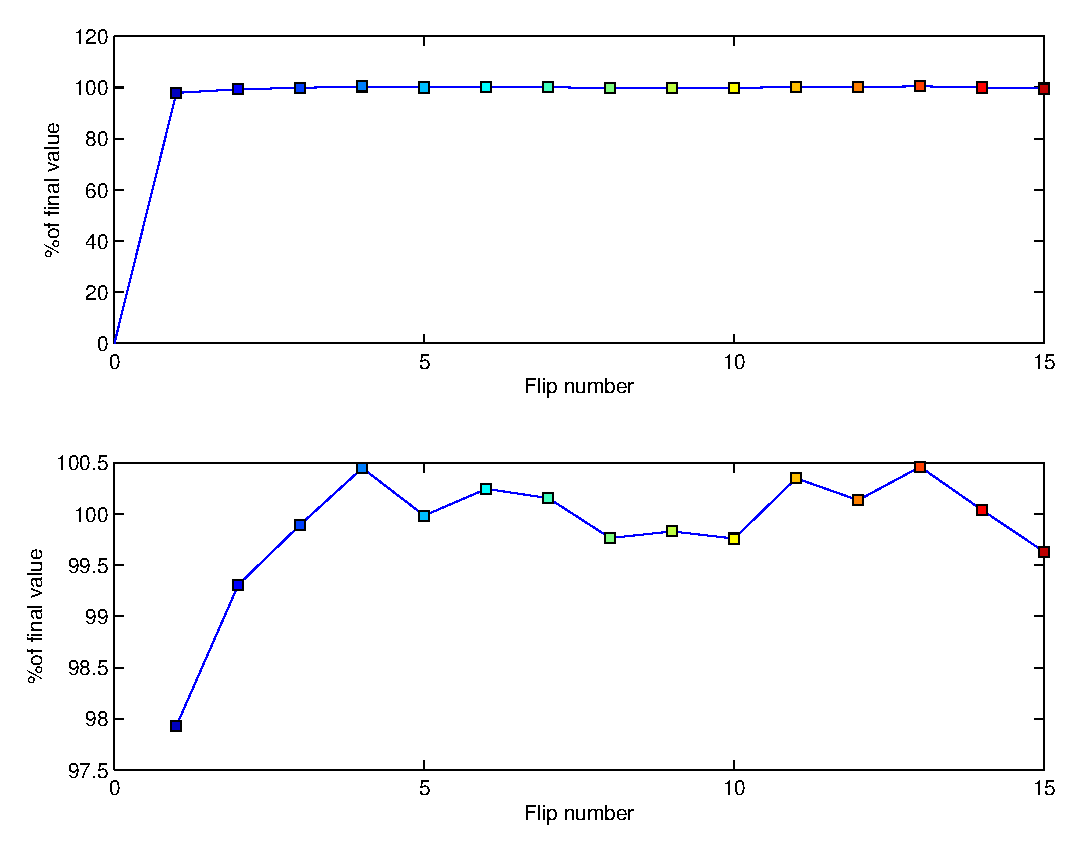
\includegraphics[width=0.7\textwidth]{torquer-multiflip}
    \caption{Torquer saturation}
    \label{fig:satWV}
\end{figure}

\Cref{fig:satWV} shows how the torquer field changes as the number of flips increases. Both graphs show the same data, the graph on the bottom has been zoomed in to show the points after the first flip better. The 0\% point is found by averaging 20 samples from the beginning of the first magnetic field waveform in \cref{fig:driveWV}. The rest of the points are found by averaging the last 20 samples of the magnetic field waveforms from \cref{fig:driveWV}. The first flip gets the torquer field to within 97\% of the final value and after two flips it has reached the final value. 

\subsection{Torquer Diagnostics}

Comparators are used to detect in flight if the torquers and drivers are functioning properly. One comparator is used to determine if the capacitor is charged and another is used to detect if the capacitor is discharged. The comparators are checked both before and after a torquer flip to see if the capacitor was charged before an attempted flip and discharged after. If the capacitor did not discharge then the torquer did not flip probably because of a bad connection somewhere. This information is logged in flight and can be used on the ground to analyze how well the torquers are working.

\todo[inline]{Need some discussion of what is done with the info but also need to figure out what should be done.}


\section{Sensors}

The only sensor called out in \cite{Mentch11} was a magnetometer. The accuracy of the magnetometer was not specified but it needs to be able to determine rotation rates accurately enough for the \ac{ACDS} to work.

\subsection{Magnetometer}

The magnetometers on the satellite are Honeywell HMC1052 \ac{AMR} sensors. These sensors use \ac{AMR} elements in a bridge configuration to measure the field in each axis. The HMC1052 is a 2-axis sensor that measures the field in the axis that are parallel to the board that it is mounted on (X and Y). Each face of \ac{ARC} will have a single HMC1052 giving a total of 4 measurements in each axis.

The magnetometers are located on the back of the \acs{SPB}, shown in \cref{fig:SPB}. The magnetometer, with surrounding circuitry, is visible on the back of the board as are the ADC and amplifier. An accelerometer is also located on the back of the solar panel board and is used for a different mission objective. The data connector powers the sensors, including a temp sensor (not shown), and provides access to the sensor data.

\subsubsection{Magnetometer Amplifier}

\todo[inline]{This is mostly for my reference. Should it be here?}

The \ac{SPB} also contains an amplifier to amplify the magnetometer signal before it is read by the \ac{ADC}. This allows the output voltage of the magnetometer to fill the input range of the \ac{ADC}. The required range of the magnetometer will be largely dependent on the torquer geometry and could be more then the $\pm$600 mGuass or so of earths field. The amplifier can be used to trade range for resolution depending on what is needed.

The gain for the amplifier can be calculated as follows: If the maximum output range of the sensor is restricted to $\pm$ 4 Gauss. With a bridge voltage of 3.3 V and a sensitivity of 1 mV/V/Gauss this results in a $\pm$ 13.2 mV voltage swing. The bridge offset is $\pm$ 1.25 mV/V or $\pm$ 4.125 mV. This results in a total possible swing of $\pm$ 17.325 mV. The input voltage range of the \ac{ADC} is $\pm$ 1.65 V. This results in a gain of about 95. 

\subsubsection{Magnetometer \acl{ADC}}

Each magnetometer has its own \ac{ADC} on each \ac{SPB}. The \ac{ADC} used is the LTC2487. The LTC2487 is a 16-bit delta sigma \ac{ADC} that has two differential analog input channels and an \ac{I2C} interface. For a bridge voltage of 3.3V the HMC1052 has a sensitivity 3.3mV/Gauss. If the amplifier gain is 95 this results in a sensitivity of 0.31V/Gauss. For a 3.3V reference voltage the \ac{ADC} has a resolution of $25 \mu V$ this results in a resolution of 81 $\mu$Gauss / LSB.

\subsubsection{Magnetometer Operation}
%\subsection{\acs{AMR} Background}

The HMC1052 sensors used on the \ac{ACDS} are \ac{AMR} sensors. They work by having a bridge with 4 elements that all change resistance with the applied magnetic field. The \ac{AMR} sensors are primarily sensitive to magnetic fields in their sensitive direction, ($H_s$), but they are also slightly sensitive to magnetic fields in an axis normal to the sensitive direction, ($H_C$), called the cross axis. The sensor is only sensitive to magnetic fields that are in the film plane of the \ac{AMR} sensor. For the 2-axis HMC1052 this means that both sensors show some sensitivity to fields in both the X and Y axes. The cross axis effect varies from sensor to sensor \todo[disable]{Test this} so calibration values must be calculated for each sensor \cite{AN215}.

\Cref{eq:magcross} shows the simplified equation for the magnetometer as described in \cite{AN215}. $V_b$ is the bridge voltage that is applied to the sensor. $S_s$ is the sensitivity in the sensitive direction. D is the cross field sensitivity offset. The HMC1052 datasheet\cite{HMC1052} mentions that the sensors have a bridge offset. The bridge offset is the sensor output when zero field is applied to the sensor and can be a large as \textpm1.25 Gauss. The bridge represented by $V_{os}$ in \cref{eq:magcross}.

\begin{equation}
    V_s = V_b \left(S_s H_s + D \cdot H_c + V_{os} \right)
    \label{eq:magcross}
\end{equation}
 
The bridge voltages are measured using an \ac{ADC} that uses the bridge voltage as its reference. To take this into account and simplify the equations, the following substitution is made:
\begin{equation}
    V_s'=\frac{V_s}{V_b}
    \label{eq:adcsub}
\end{equation}

\Cref{eq:magcross} is useful to determine the voltage that would be produced for a given magnetic field condition, but not if the sensor voltages are known but the fields are not.

Because the calculated field in the sensitive direction also depends on the field in the cross axis direction, \cref{eq:magcross} was duplicated for the cross field sensor voltage and both equations were solved simultaneously. This resulted in twice as many constants as \cref{eq:magcross}. The voltages $V_s'$ and $V_c'$ are the normalized \ac{ADC} voltages in the sensitive and cross axis respectively. Each of the constants from \cref{eq:magcross} has similar duplicate forms that comes from the extra equation that was used to solve for $H_s$. To distinguish the constants additional subscripts have been added. \Cref{eq:magsolved} shows \cref{eq:magcross} solved for the unknown quantity, $H_s$.

\begin{equation}
    \begin{split}
    H_s = & \frac{V'_s }{{S_s}_s - \frac{D_s \cdot D_c}{{S_s}_c}} - \frac{D_s \cdot  V'_c }{{S_s}_c \cdot {S_s}_s - D_s \cdot D_c}\\
    & {}- \frac{{S_s}_c \cdot {V_{os}}_s  -D_s \cdot {V_{os}}_c}{{S_s}_c \cdot {S_s}_s - D_s \cdot D_c}
    \end{split}
    \label{eq:magsolved} 
\end{equation}

\Cref{eq:magsolved} can be used to calculate the magnetic field from measured voltages, but the relationship between the constants is complex. To simplify \cref{eq:magsolved} the constants can be consolidated to get \cref{eq:magcal}.

\begin{equation}
    \label{eq:magcal}
    \begin{split}
        H_s &= C_1 \cdot V_s' + C_2 \cdot V_c' + C_3\\
        H_c &= C_4 \cdot V_s' + C_5 \cdot V_c' + C_6
    \end{split}
\end{equation}

In this case $V_s'$ and $V_c'$ are the \ac{ADC} values for the cross and sensitive axes, respectively. $C_1$, $C_2$, $C_4$, and $C_5$ are the sensitivity in the sensitive and cross directions and $C_3$ and $C_6$ correct for the bridge offset of the sensor and also compensates for external offsets. These offset values are used to correct for the torquer offsets.

\subsubsection{Magnetometer Calibration}
\label{sec:magcal}

To calibrate the magnetometer, the coefficients in \cref{eq:magcal} must be calculated. The magnetometer is first placed inside the Helmholtz Cage. The field is set under MATLAB control so the entire calibration process can run automatically. The calibration program sweeps the field inside the Helmholtz Cage through a predefined sequence and reads the sensor output at each point. 

The method of least squares is used to solve \cref{eq:magmat} for the coefficients in \cref{eq:magcal}. Each line in the $\matt{A}$ matrix represents a separate magnetic field measurement. $H_n$ is the $n^{\text{\tiny th}}$ value set by the Helmholtz cage in the sensitive axis. 

\begin{equation}
    \label{eq:magmat}
    \begin{split}
    \vect{b}&=\matt{A} \vect{x} \\
    {\text{\raggedright where}} \\
    \vect{b}&= 
    \begin{bmatrix}
        H_1 \\
        \vdots \\
        H_n \\
    \end{bmatrix} \\
    \matt{A}&=
    \begin{bmatrix}
        {V_s}_1 & {V_c}_1 & 1 \\
        \vdots & \vdots & \vdots\\
        {V_s}_n & {V_c}_n & 1 \\
    \end{bmatrix} \\
    \vect{x}&= 
    \begin{bmatrix}
        C_1 \\
        C_2 \\
        C_3 \\
    \end{bmatrix} 
    \end{split}
\end{equation}

The least squared solution minimizes the error across all data points. This results in calibration values that minimize error across the range of calibration points that were taken. This means that the points used to do the calibration should span the range of values that the magnetometer is expected to measure. 

\subsection{\acs{MEMS} Gyros}

For flight a \ac{MEMS} gyro will also be used to sense rotation rates. The \ac{MEMS} gyro does not have that great resolution compared to what can be achieved with the magnetometer \todo{Perhaps should have some sort of evidence for this}. The gyro does, however directly read the rotation rate so it is good for quickly giving a rough idea of the rotation rates of the satellite. If the satellite is rotating fast enough the magnetometer readings will alias and it can appear that the satellite is rotating at a speed that is much less than the actual speed. If the rotation rates are too high for the \ac{MEMS} gyro the output will saturate and while the rotation rates are not measurable a direction and lower bound can be determined.


\section{Embedded System}

At the heart of the \ac{ACDS} is an embedded system. This system is responsible for running the algorithm, taking housekeeping data and, interfacing with the rest of the satellite.

\subsection{Processor}

The processor used for the \ac{ACDS} and all systems on \ac{ARC} is the MSP430f2618. The MSP430 is a microcontroller aimed at low power applications. The MSP430f2618 runs at a maximum speed of 16MHz and has 8kB of RAM and 116kB of flash memory. The MSP430 microcontrollers do not have an external memory bus so there is no good way to add extra memory or program storage. 

\subsection{SD card}

For flight data storage a SD card is used. This is necessary because of the needed space and write times. The internal flash is limited and also needs to be used for program storage making it undesirable for data storage. Furthermore the internal flash can't be read while it is being written. Because the write times for the internal flash are fairly slow this would disrupt the operation of the program and is not desirable except for the occasional data writes.

\subsection{\acs{ARC} Bus Communication}

The sensor data is read by the \ac{LEDL} board and sent over the bus to the \ac{ACDS} board. The \ac{ACDS} board initiates the connection by sending a command to tell how often measurements should be sent. The \ac{LEDL} then takes sensor data and sends it at the requested interval.

\section{Board Layout}

\Cref{fig:3dview} shows the \ac{ACDS} system. The X and Y axis torquers are shown on the board as well as the pull pin and header. The header and pull pin locations are more or less fixed which doesn't leave much wiggle room for where to place the torquers.

\begin{figure}[H]
    \centering
    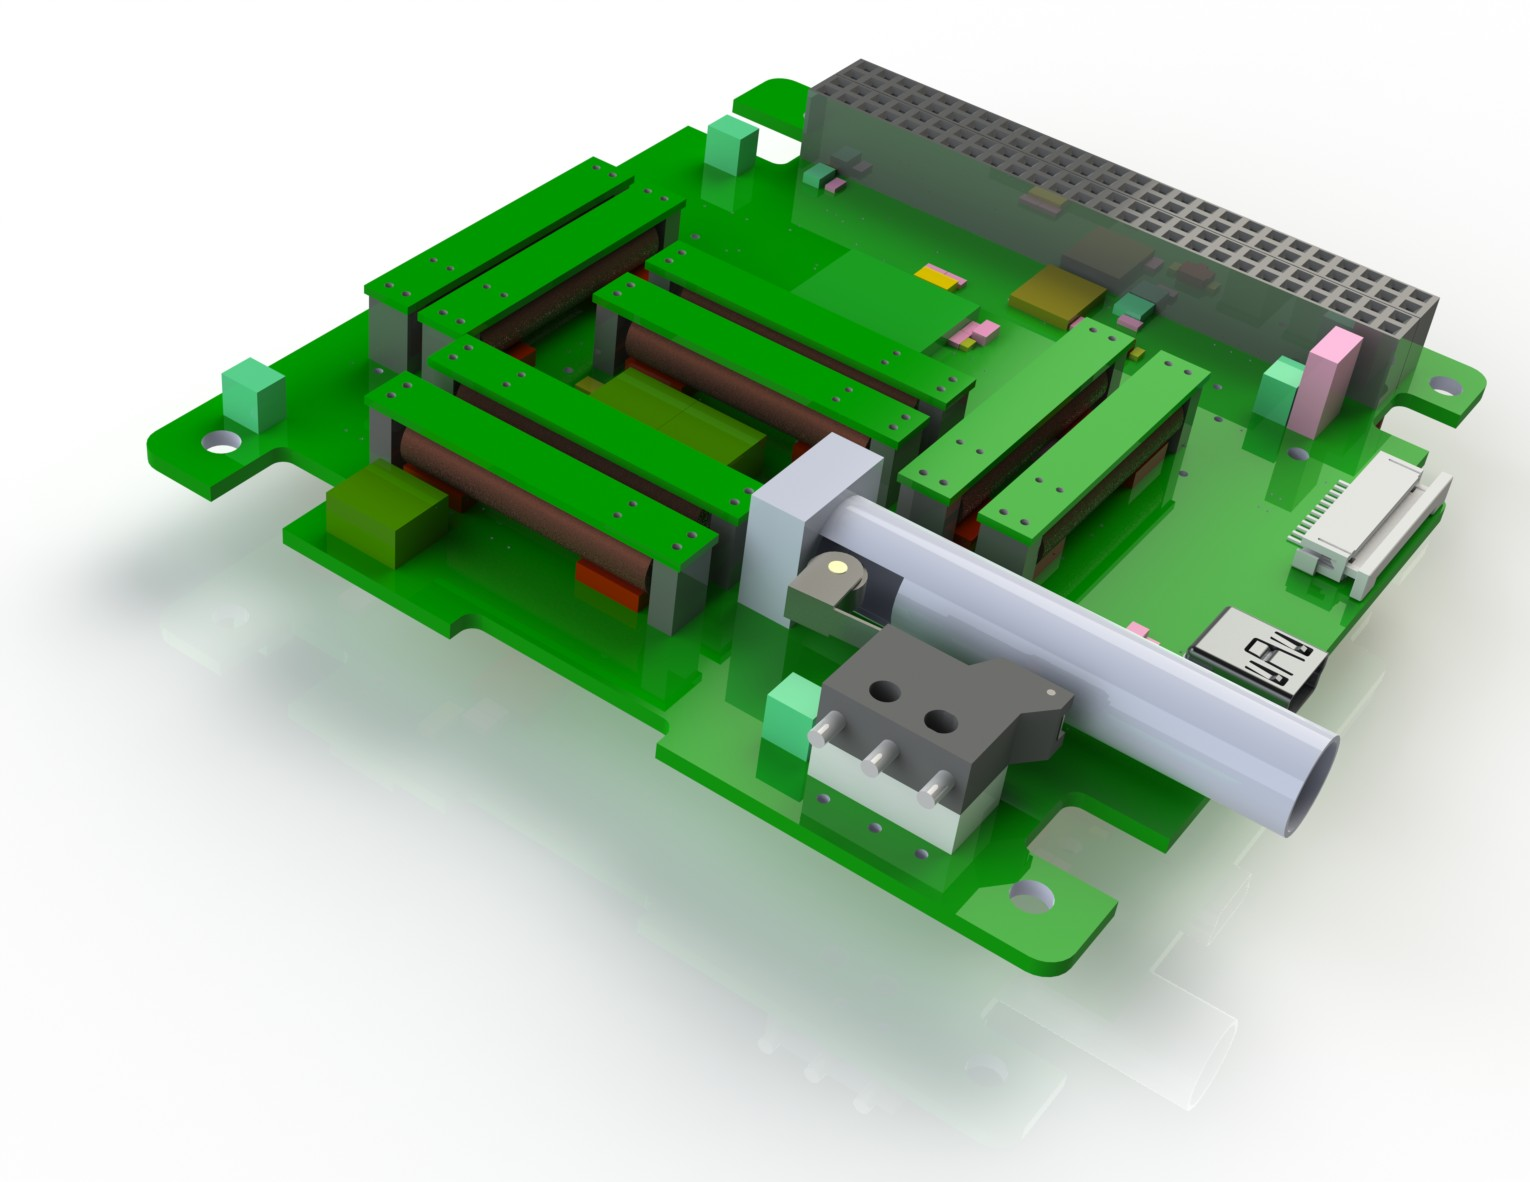
\includegraphics[width=0.8\textwidth]{board-drawing}
    \caption{3D view of the CubeSat \acs{ACDS} system}
    \label{fig:3dview}
\end{figure}

\begin{comment}
\begin{figure}[H]
    \centering
    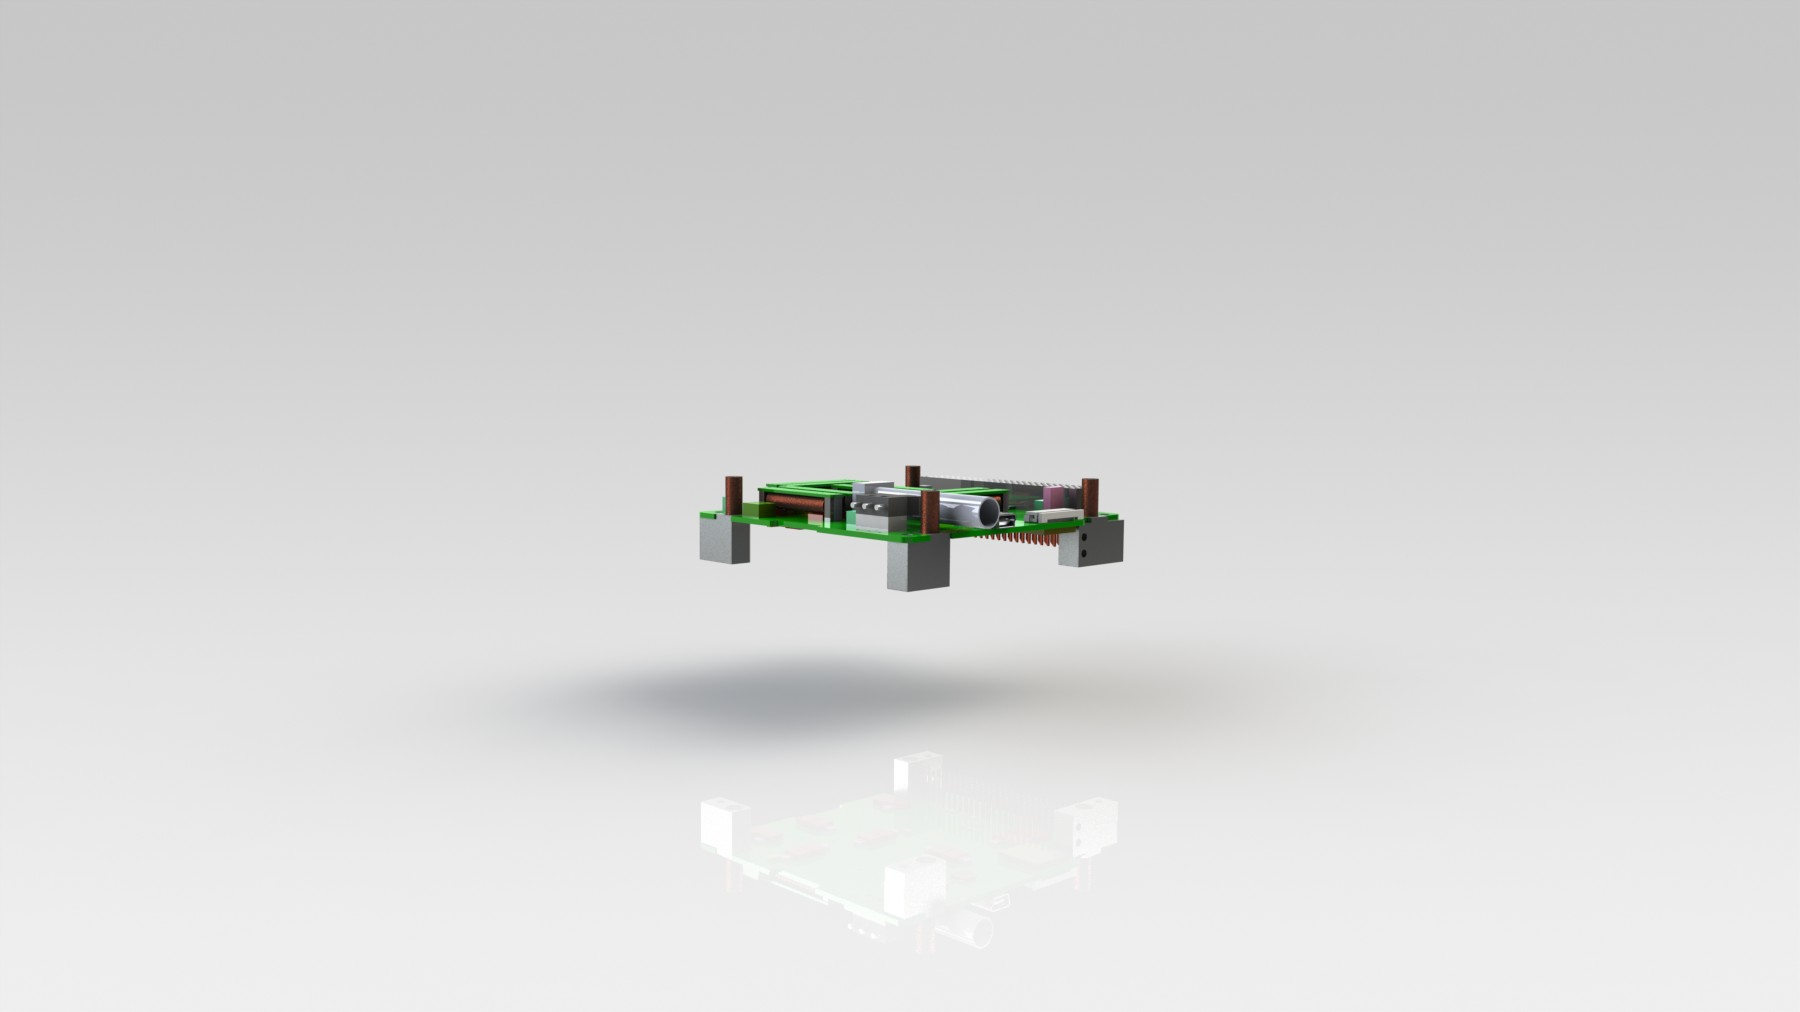
\includegraphics[width=0.8\textwidth]{board-drawing-with-standoffs}
    \caption{3D view of the CubeSat \acs{ACDS} system with Z-axis torquers}
\end{figure}
\end{comment}

\begin{comment}

The \ac{ACDS} board is a four layer board with the inner layers as power and ground planes. \Cref{fig:layout} shows the \ac{PCB} layout for the \ac{ACDS} board. The circuitry is very repetitive and this was used when the board was laid out. A quick switching time is desired and moderate currents are involved, the lines to and from the \acp{MOSFET} were kept as short as possible. The power plane is split so that there is a 3.3V plane underneath the MSP430 and a $V_{batt}$ plane elsewhere.

\begin{figure}[H]
    \centering
    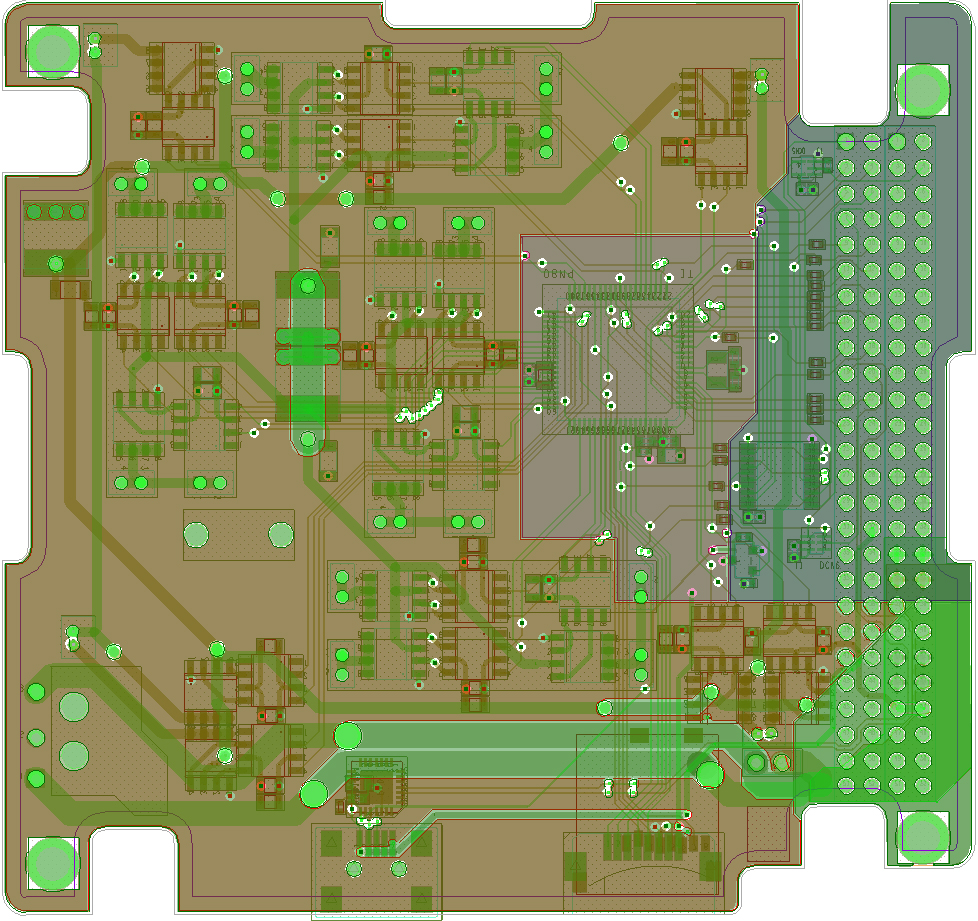
\includegraphics[width=0.8\textwidth]{board-design}
    \caption{Board Layout for the CubeSat \acs{ACDS} system}
    \label{fig:layout}
\end{figure}

\end{comment}
